\documentclass[aspectratio=169,10pt]{beamer}

% --- Ngôn ngữ & Font Tiếng Việt ---
\usepackage[utf8]{inputenc}
\usepackage[T5]{fontenc}
\usepackage{amsmath,amssymb,amsfonts}
\usepackage{graphicx}
\usepackage{booktabs}
\usepackage{tabularx}
\usepackage{tikz}
\usetikzlibrary{arrows.meta,positioning,shapes.geometric,fit,calc}

% --- Cấu hình Theme Beamer Hiện Đại & Chuyên Nghiệp ---
\usetheme{Madrid}
\usefonttheme{professionalfonts}

% --- Bảng Màu Công Nghiệp (Industrial AMR Palette) ---
\definecolor{NavyBlue}{RGB}{18, 48, 86}      % Màu xanh đậm chủ đạo
\definecolor{SteelBlue}{RGB}{35, 95, 145}     % Màu xanh thép phụ
\definecolor{SafetyOrange}{RGB}{230, 105, 0}  % Màu cam an toàn công nghiệp
\definecolor{DarkSlate}{RGB}{30, 35, 42}      % Màu xám đen
\definecolor{LightGrey}{RGB}{245, 247, 250}   % Nền khối xám nhạt
\definecolor{AccentGreen}{RGB}{28, 130, 60}   % Xanh lá thành công

\setbeamercolor{palette primary}{bg=NavyBlue,fg=white}
\setbeamercolor{palette secondary}{bg=SteelBlue,fg=white}
\setbeamercolor{palette tertiary}{bg=NavyBlue!90,fg=white}
\setbeamercolor{palette quaternary}{bg=DarkSlate,fg=white}

\setbeamercolor{structure}{fg=NavyBlue}
\setbeamercolor{titlelike}{parent=palette primary,fg=NavyBlue}
\setbeamercolor{frametitle}{bg=NavyBlue,fg=white}
\setbeamercolor{author in head/foot}{bg=NavyBlue!90,fg=white}
\setbeamercolor{title in head/foot}{bg=SteelBlue,fg=white}
\setbeamercolor{date in head/foot}{bg=DarkSlate,fg=white}

% Cấu hình khối thông tin (Blocks)
\setbeamercolor{block title}{bg=NavyBlue,fg=white}
\setbeamercolor{block body}{bg=LightGrey,fg=DarkSlate}
\setbeamercolor{block title example}{bg=SteelBlue,fg=white}
\setbeamercolor{block body example}{bg=LightGrey,fg=DarkSlate}
\setbeamercolor{block title alerted}{bg=SafetyOrange,fg=white}
\setbeamercolor{block body alerted}{bg=SafetyOrange!10,fg=DarkSlate}

\setbeamertemplate{navigation symbols}{} % Ẩn thanh icon navigation
\setbeamertemplate{caption}[numbered]
\setbeamertemplate{footline}[frame number]

% Thiết lập thư mục ảnh
\graphicspath{{figures/}}

% --- Thông tin Trang bìa ---
\title[\textbf{Factory Delivery AMR}]{\textbf{\LARGE FACTORY DELIVERY AMR}}
\subtitle{\large Robot Di Động Tự Hành Vận Chuyển Linh Kiện Nhà Máy\\{\small \textbf{Động học $\cdot$ Động lực học $\cdot$ Điều khiển PID $\cdot$ Mô phỏng ROS 2 \& Gazebo}}}
\author[\textbf{Nguyễn Hoàng Anh}]{\textbf{Tác giả:} Nguyễn Hoàng Anh\\[2pt]{\small Nhóm Dự án Industrial AMR Robot}}
\institute[\textbf{Industrial AMR}]{\textbf{Khoa Cơ Điện Tử \& Kỹ Thuật Robot}}
\date[\textbf{10/11/2026}]{Ngày 10 tháng 11 năm 2026}

\begin{document}

% ==============================================================================
% SLIDE 1: TRANG BÌA (TITLE SLIDE)
% ==============================================================================
\begin{frame}[plain]
    \begin{tikzpicture}[remember picture,overlay]
        \fill[NavyBlue] (current page.north west) rectangle ($(current page.north east)+(0,-1.4cm)$);
        \fill[SafetyOrange] ($(current page.north west)+(0,-1.4cm)$) rectangle ($(current page.north east)+(0,-1.48cm)$);
    \end{tikzpicture}
    \vspace{0.4cm}
    \begin{columns}[c]
        \begin{column}{0.55\textwidth}
            \vspace{-0.2cm}
            {\color{NavyBlue}\Huge \textbf{FACTORY DELIVERY}}\\[2pt]
            {\color{SafetyOrange}\Huge \textbf{AMR ROBOT}}\\[8pt]
            {\large \textbf{Robot Tự Hành Vận Chuyển Linh Kiện}}\\[10pt]
            \begin{beamercolorbox}[rounded=true,shadow=false,wd=\textwidth,sep=5pt]{block body}
                \small
                $\bullet$ \textbf{Thiết kế cơ điện tử:} Tham số hóa OpenSCAD\\
                $\bullet$ \textbf{Lý thuyết điều khiển:} Động học vi sai \& PID\\
                $\bullet$ \textbf{Mô phỏng:} ROS 2 Humble \& Gazebo Harmonic
            \end{beamercolorbox}
            \vspace{8pt}
            {\small \textbf{Thực hiện:} Nguyễn Hoàng Anh}\\[1pt]
            {\footnotesize \textit{Nhóm Phát Triển Industrial AMR Robot}}
        \end{column}
        \begin{column}{0.43\textwidth}
            \centering
            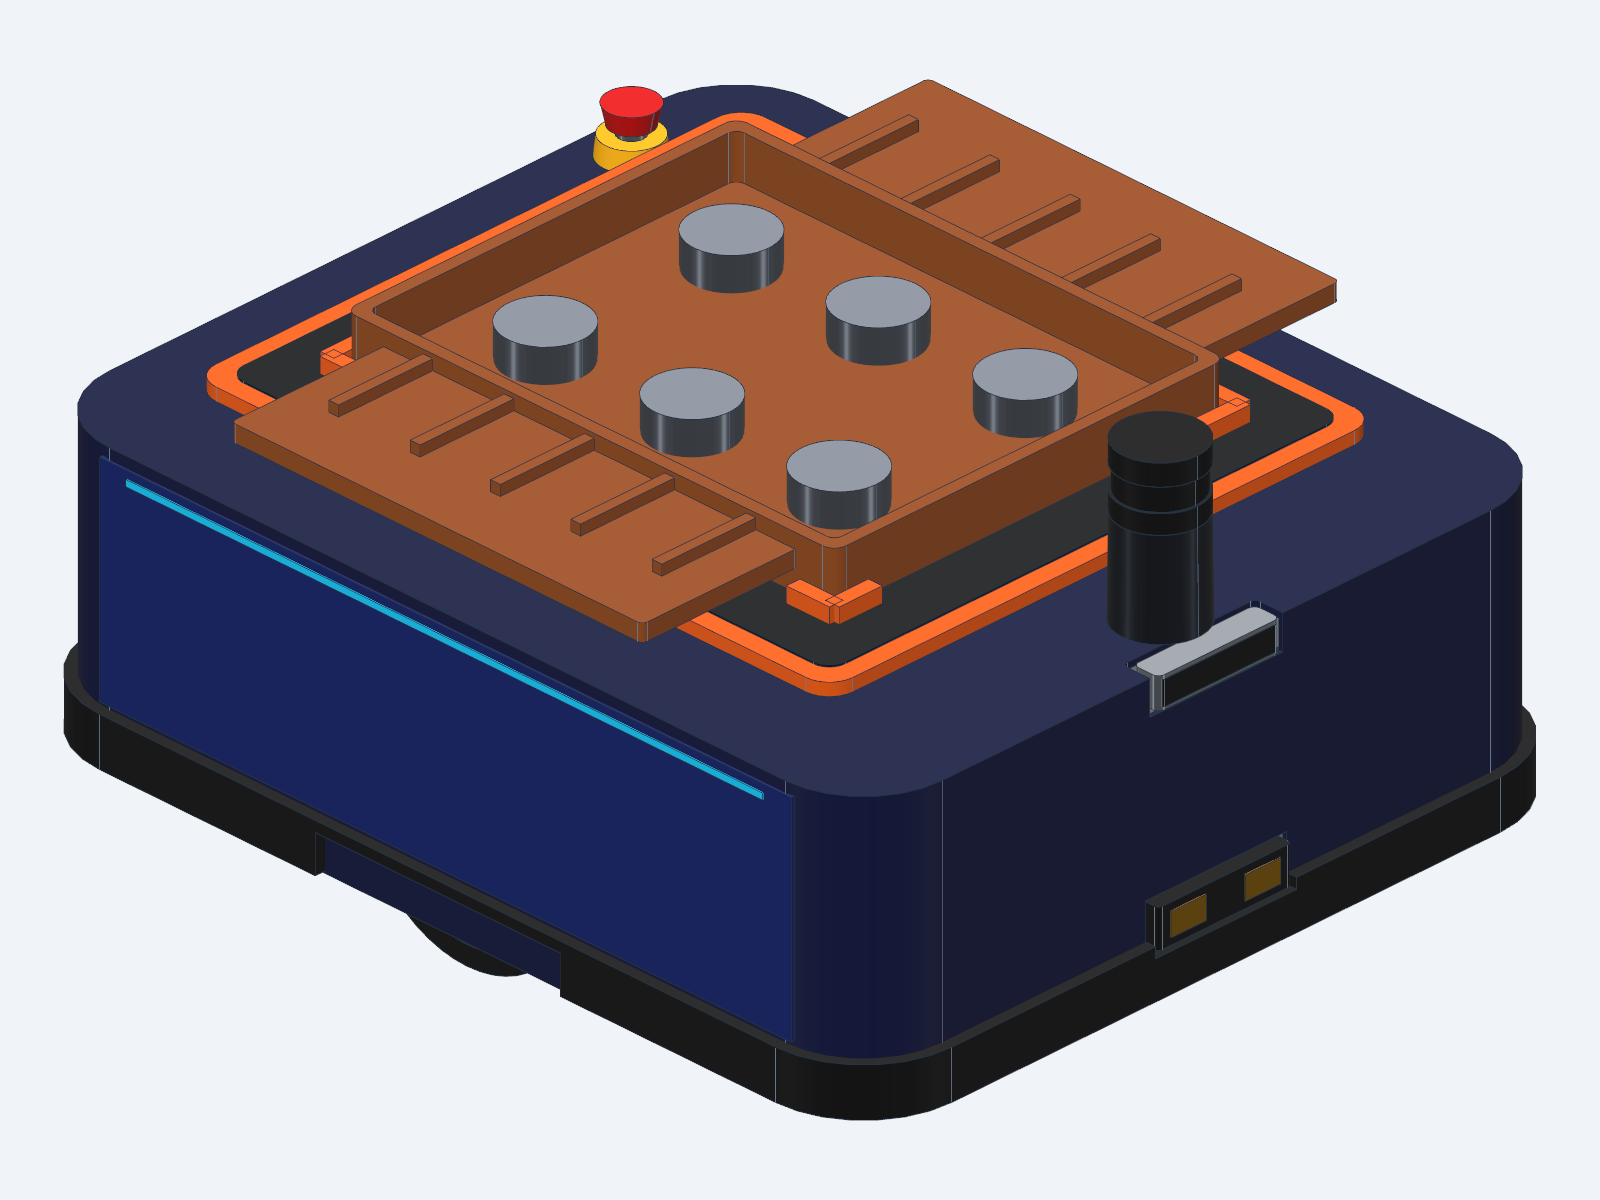
\includegraphics[width=\textwidth,height=0.68\textheight,keepaspectratio]{amr_assembled.png}\\[2pt]
            {\scriptsize \textit{Mô hình 3D hoàn chỉnh trong OpenSCAD}}
        \end{column}
    \end{columns}
\end{frame}

% ==============================================================================
% SLIDE 2: BÀI TOÁN & YÊU CẦU KỸ THUẬT
% ==============================================================================
\begin{frame}{1. Đặt Vấn Đề \& Yêu Cầu Kỹ Thuật (KPIs)}
    \begin{columns}[T]
        \begin{column}{0.50\textwidth}
            \begin{block}{\small \textbf{Bối Cảnh Bài Toán Nhà Máy X}}
                \scriptsize
                \begin{itemize}
                    \item \textbf{Nhiệm vụ:} Nhận khay linh kiện tại \textbf{Kho A}, tự hành vận chuyển qua các trạm \textbf{B $\rightarrow$ C $\rightarrow$ D}.
                    \item \textbf{Khép kín:} Tự động quay về trạm sạc sau khi hoàn tất chu trình hoặc khi điện áp dưới ngưỡng an toàn.
                    \item \textbf{Phối hợp người - máy:} Tránh vật cản tĩnh và động theo thời gian thực trong hành lang nhà xưởng.
                \end{itemize}
            \end{block}
            \vspace{-4pt}
            \begin{center}
                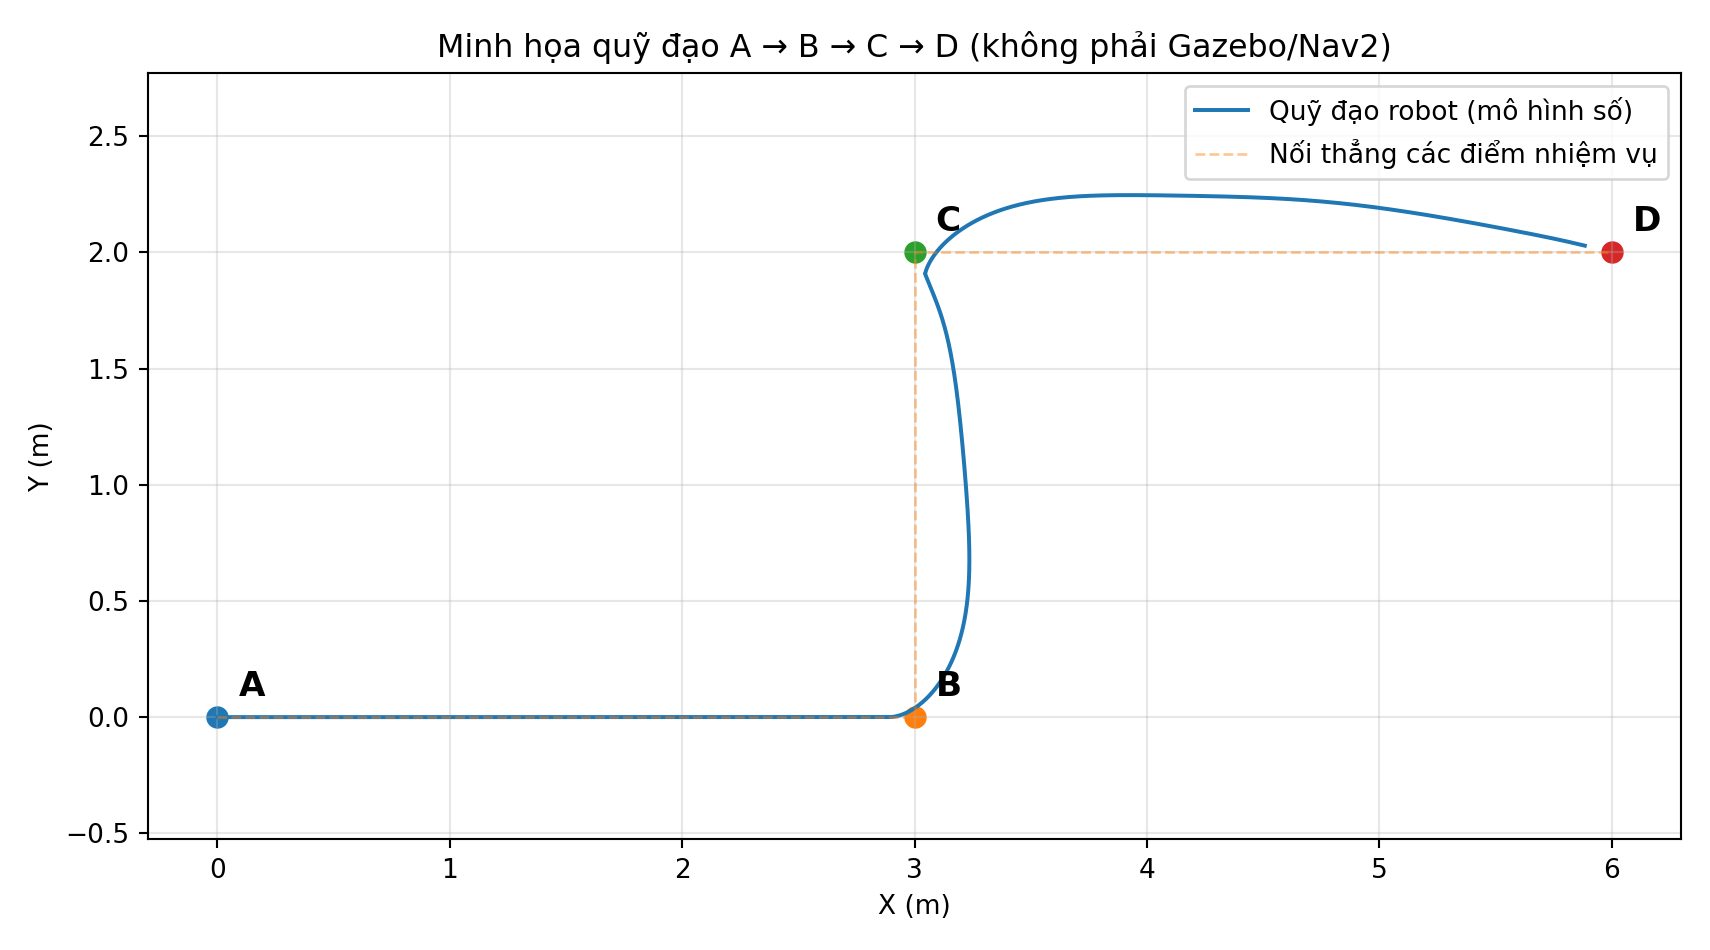
\includegraphics[width=0.95\textwidth,height=0.20\textheight,keepaspectratio]{extended_waypoint_abcd.png}\\[1pt]
                {\tiny \textit{Sơ đồ quỹ đạo nhiệm vụ vận chuyển qua các Waypoint A-B-C-D}}
            \end{center}
        \end{column}
        
        \begin{column}{0.48\textwidth}
            \begin{block}{\small \textbf{Chỉ Số Kỹ Thuật Yêu Cầu (Target KPIs)}}
                \tiny
                \centering
                \begin{tabularx}{\textwidth}{Xcr}
                    \toprule
                    \textbf{Thông số kỹ thuật} & \textbf{Chỉ số yêu cầu} & \textbf{Ghi chú kiểm tra} \\
                    \midrule
                    Tải trọng hữu ích (Payload) & \textbf{20 kg} & Khay linh kiện chuẩn \\
                    Chiều rộng hành lang & $\ge$ \textbf{1,20 m} & Bán kính quay tối ưu \\
                    Tốc độ di chuyển tối đa & $\ge$ \textbf{1,20 m/s} & Đảm bảo tiến độ dây chuyền \\
                    Sai số dừng vị trí (Docking) & $\le$ \textbf{$\pm$30 mm} & Khớp tiếp xúc chân kệ/sạc \\
                    Thời gian hoạt động liên tục & $\ge$ \textbf{4,0 giờ} & Pin LiFePO4 48V-30Ah \\
                    Cơ chế an toàn & \textbf{Đa tầng} & LiDAR + Bumper + E-stop \\
                    \bottomrule
                \end{tabularx}
            \end{block}
            \vspace{-3pt}
            \begin{alertblock}{\scriptsize \textbf{Ràng Buộc Thiết Kế Cơ Bản}}
                \tiny
                Robot phải tự xoay tại chỗ ($360^\circ$) để quay đầu trong hành lang hẹp 1,2 m mà không gây va quệt thành vách.
            \end{alertblock}
        \end{column}
    \end{columns}
\end{frame}

% ==============================================================================
% SLIDE 3: KIẾN TRÚC HỆ THỐNG PHÂN TẦNG (SYSTEM ARCHITECTURE)
% ==============================================================================
\begin{frame}{2. Kiến Trúc Hệ Thống Phân Tầng}
    \begin{columns}[T]
        \begin{column}{0.54\textwidth}
            \begin{block}{\small \textbf{Mô Hình 4 Tầng Chức Năng (Layered Architecture)}}
                \scriptsize
                \textbf{Tầng 1: Quản lý Nhiệm vụ (Mission Layer)}\\
                $\bullet$ State Machine: Điều phối logic di chuyển Kho A $\rightarrow$ B $\rightarrow$ C $\rightarrow$ D.\\
                $\bullet$ Giám sát mức pin \& điều phối lệnh quay về trạm sạc.\\
                \textbf{Tầng 2: Định vị \& Điều hướng (Navigation \& Perception)}\\
                $\bullet$ Định vị SLAM (Cartographer/AMCL) kết hợp Sensor Fusion (EKF).\\
                $\bullet$ Lập kế hoạch đường đi toàn cục \& cục bộ tránh vật cản (Nav2).\\
                \textbf{Tầng 3: Điều khiển Chuyển động (Control Layer)}\\
                $\bullet$ Tính toán động học nghịch: $(v, \omega) \rightarrow (\dot{\varphi}_R^*, \dot{\varphi}_L^*)$.\\
                $\bullet$ Vòng kín PID tốc độ bánh xe tần số cao trên ESP32-S3.\\
                \textbf{Tầng 4: Phần cứng \& Chấp hành (Hardware Layer)}\\
                $\bullet$ Động cơ BLDC, Khung gầm vi sai 2 bánh + 4 caster, Cảm biến.
            \end{block}
        \end{column}
        
        \begin{column}{0.44\textwidth}
            \begin{block}{\small \textbf{Phân Rã 11 Module Hệ Thống}}
                \tiny
                \begin{tabularx}{\textwidth}{llX}
                    \toprule
                    \textbf{Mã} & \textbf{Module} & \textbf{Vai trò cốt lõi} \\
                    \midrule
                    \textbf{M1} & Mechanical & Khung gầm 2 tầng, bàn nâng chữ X \\
                    \textbf{M2} & Drive System & 2 Động cơ BLDC + 4 bánh Caster 360$^\circ$ \\
                    \textbf{M3} & Sensor & 2D LiDAR, RealSense D455, IMU, Encoder \\
                    \textbf{M4} & Localization & EKF Sensor Fusion (Odom + IMU + AMCL) \\
                    \textbf{M5} & Navigation & Global/Local Planner (Nav2 Stack) \\
                    \textbf{M6} & Obstacle & Vùng an toàn 3 cấp (An toàn/Cảnh báo/Dừng) \\
                    \textbf{M7} & Control & Bộ điều khiển số PID trên Vi điều khiển \\
                    \textbf{M8} & Power & Pin 48V-30Ah, Smart BMS, Trạm sạc tự động \\
                    \textbf{M9} & Mission & Quản lý trạng thái và hàng đợi nhiệm vụ \\
                    \textbf{M10} & Safety & Nút E-stop, Cản va chạm, Rơ le an toàn \\
                    \textbf{M11} & Comms & CAN Bus, UART, DDS ROS 2 qua Wi-Fi \\
                    \bottomrule
                \end{tabularx}
            \end{block}
        \end{column}
    \end{columns}
\end{frame}

% ==============================================================================
% SLIDE 4: THIẾT KẾ CƠ KHÍ 3D (OPENSCAD)
% ==============================================================================
\begin{frame}{3. Thiết Kế Cơ Khí Tham Số Hóa (OpenSCAD)}
    \begin{columns}[T]
        \begin{column}{0.52\textwidth}
            \begin{block}{\small \textbf{Đặc Trưng Thiết Kế Cơ Khí}}
                \scriptsize
                \begin{itemize}
                    \item \textbf{100\% Parametric Code:} Quản lý kích thước hình học toàn bộ bằng biến số (\texttt{cad/main.scad}), cho phép thay đổi bán kính bánh xe, bề rộng robot tức thì.
                    \item \textbf{Cấu hình bánh xe ổn định cao:} Hệ dẫn động vi sai 2 bánh chủ động đặt tại tâm hình học kết hợp \textbf{4 bánh xe tự lựa (Swivel Casters)} đặt ở 4 góc giúp triệt tiêu hoàn toàn rung lắc khi nâng tải.
                    \item \textbf{Bàn nâng chữ X (Scissor Lift):} Dẫn động bằng xy-lanh điện tuyến tính, hành trình nâng 0 $\rightarrow$ 290 mm nâng khay hàng 20 kg.
                    \item \textbf{Khung gầm 2 tầng:} Thép tấm dày 6 mm sơn tĩnh điện, tối ưu khoang chứa điện tử và pin 48V.
                \end{itemize}
            \end{block}
            \vspace{-4pt}
            \begin{exampleblock}{\tiny \textbf{Thông số hình học chính}}
                \tiny $850 \times 580 \times 320\text{ mm}$ $\mid$ Bánh chủ động: $\varnothing 220\text{ mm}$ (Lốp PU, mâm CNC) $\mid$ Chiều cao nâng tối đa: $610\text{ mm}$.
            \end{exampleblock}
        \end{column}
        
        \begin{column}{0.46\textwidth}
            \centering
            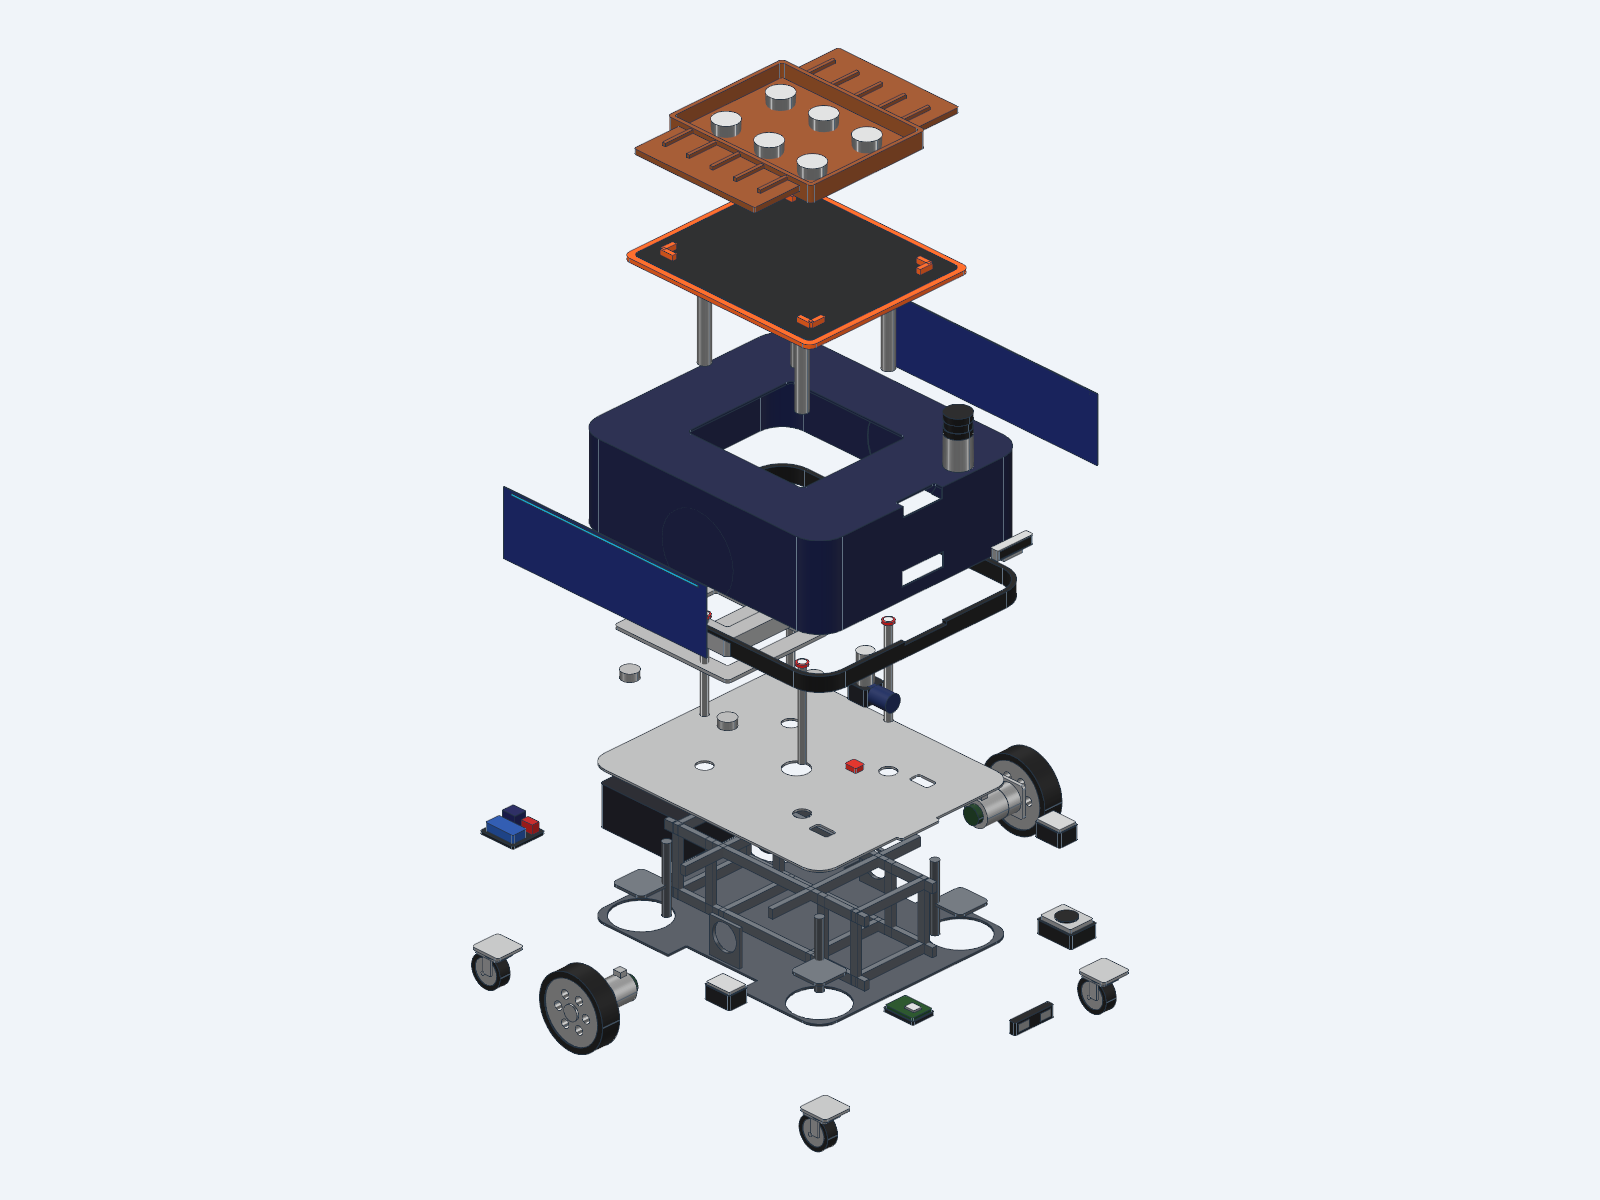
\includegraphics[width=0.92\textwidth,height=0.33\textheight,keepaspectratio]{anatomy_exploded.png}\\[1pt]
            {\tiny \textbf{Hình 4.1:} Bản vẽ phân rã giải phẫu cơ khí \& điện tử}\\[3pt]
            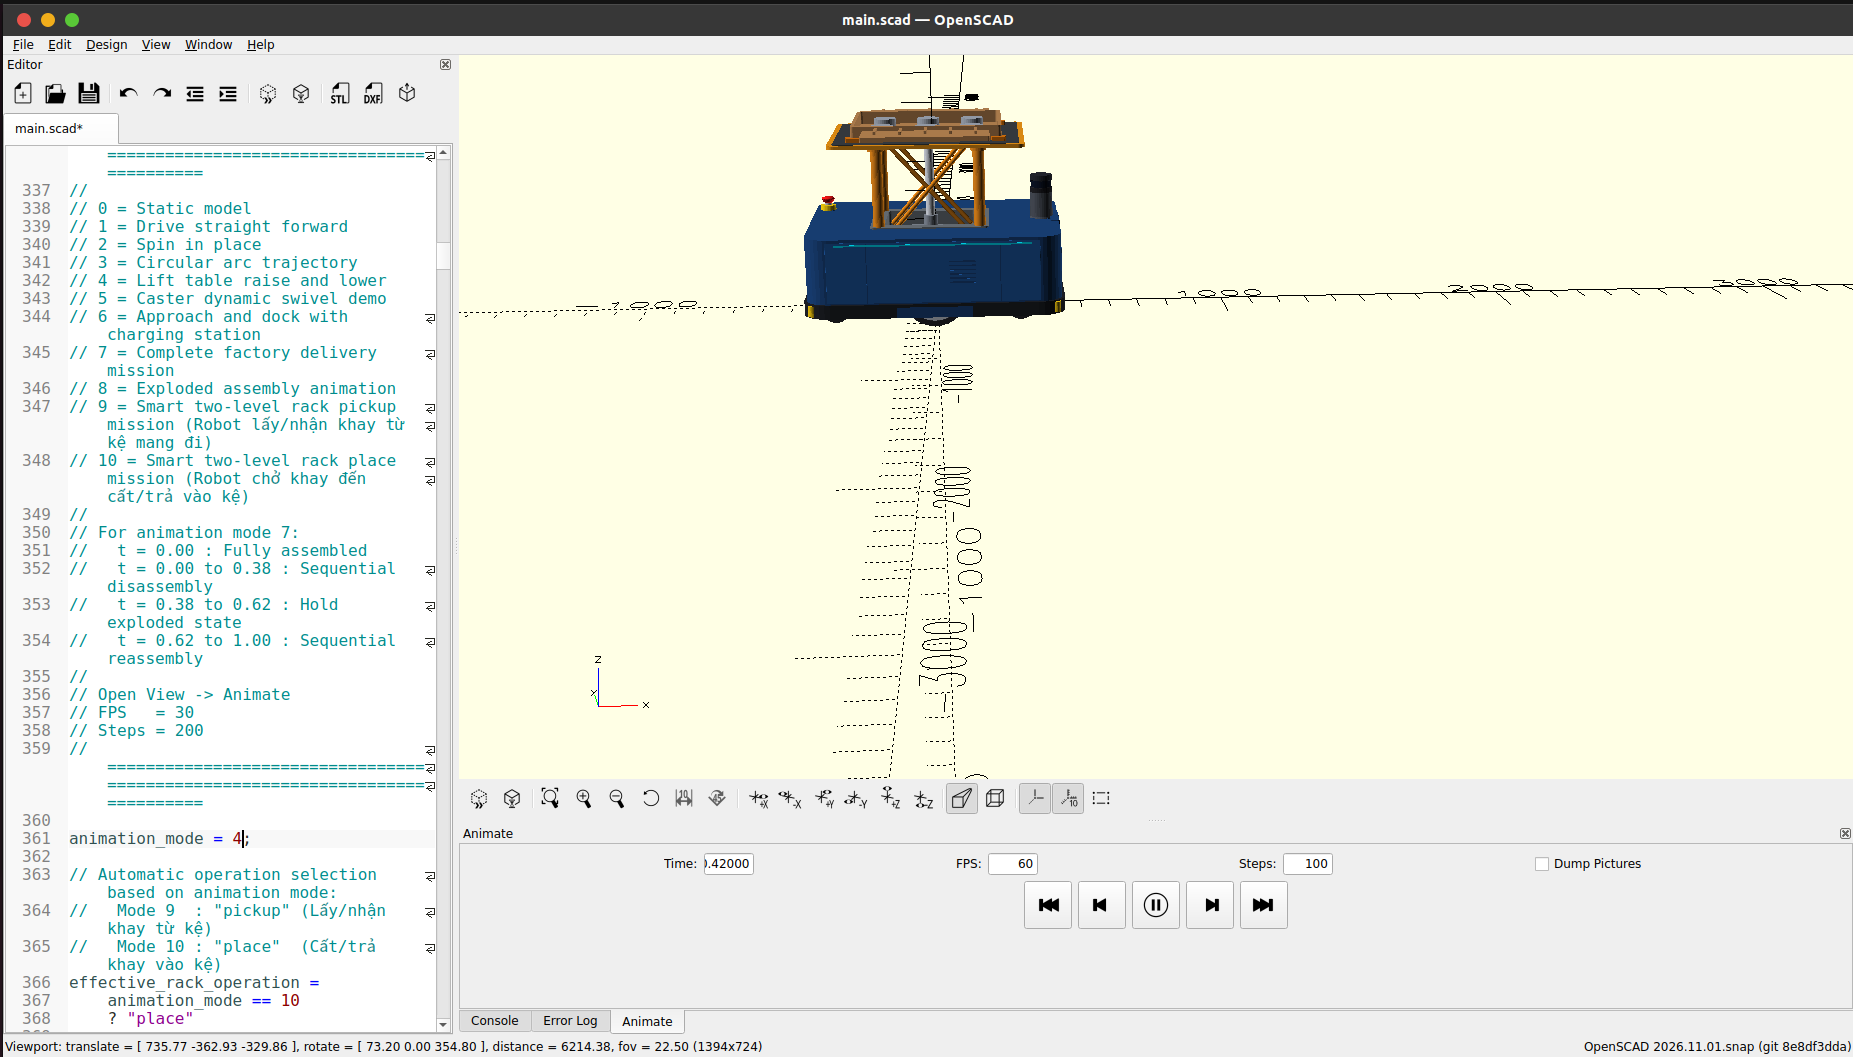
\includegraphics[width=0.85\textwidth,height=0.30\textheight,keepaspectratio]{mode_4_lift_table.png}\\[1pt]
            {\tiny \textbf{Hình 4.2:} Cơ cấu bàn nâng cắt kéo chữ X kiểm chứng trong OpenSCAD}
        \end{column}
    \end{columns}
\end{frame}

% ==============================================================================
% SLIDE 5: KIẾN TRÚC PHẦN CỨNG TOÀN DIỆN + ĐIỆN TỬ & CẢM BIẾN
% ==============================================================================
\begin{frame}{4. Kiến Trúc Phần Cứng Toàn Diện \& Hệ Thống Điện Tử}
    \begin{block}{\small \textbf{Sơ Đồ Kết Nối Phần Cứng \& Luồng Dữ Liệu Thực Thi}}
        \centering
        \begin{tikzpicture}[scale=0.72, every node/.style={transform shape, align=center}]
            % Blocks
            \node[draw=NavyBlue, fill=NavyBlue!10, rounded corners, minimum width=3.3cm, minimum height=1.2cm] (pwr) 
                {\textbf{NGUỒN NĂNG LƯỢNG}\\\scriptsize Pin LiFePO4 48V-30Ah + BMS\\\scriptsize PDU DC/DC (48V/24V/5V/3.3V)};
            
            \node[draw=NavyBlue, fill=NavyBlue!20, rounded corners, minimum width=3.5cm, minimum height=1.2cm, right=1.0cm of pwr] (sbc) 
                {\textbf{BỘ XỬ LÝ TRUNG TÂM}\\\scriptsize \textbf{NVIDIA Jetson / x86 SBC}\\\scriptsize ROS 2 $\cdot$ Nav2 $\cdot$ Cartographer};
            
            \node[draw=SteelBlue, fill=SteelBlue!20, rounded corners, minimum width=3.5cm, minimum height=1.2cm, right=1.0cm of sbc] (mcu) 
                {\textbf{VI ĐIỀU KHIỂN CẤP THẤP}\\\scriptsize \textbf{ESP32-S3 (240MHz)}\\\scriptsize Real-time Dual PID $\cdot$ E-Stop};
            
            \node[draw=DarkSlate, fill=LightGrey, rounded corners, minimum width=4.3cm, minimum height=1.4cm, below=0.7cm of sbc] (sens) 
                {\textbf{CẢM BIẾN NHẬN THỨC \& ĐO ĐẠC}\\\scriptsize $\bullet$ 2D LiDAR 360$^\circ$ (Ethernet/USB)\\\scriptsize $\bullet$ Camera Intel RealSense D455 (USB 3.0)\\\scriptsize $\bullet$ Cảm biến quán tính IMU 6-DOF (I2C)};
            
            \node[draw=SafetyOrange, fill=SafetyOrange!15, rounded corners, minimum width=4.5cm, minimum height=1.4cm, below=0.7cm of mcu] (act) 
                {\textbf{CƠ CẤU CHẤP HÀNH \& ĐỘNG CƠ}\\\scriptsize $\bullet$ 2x Driver BLDC 24V/15A + Dual Motor\\\scriptsize $\bullet$ 2x Optical/Magnetic Encoder (Feedback)\\\scriptsize $\bullet$ Xy-lanh điện bàn nâng Scissor Lift};
            
            % Arrows
            \draw[->, thick, red!80!black] (pwr.east) -- node[above, align=center]{\tiny 48V/24V} (sbc.west);
            \draw[->, thick, red!80!black] (pwr.north) -- ++(0,0.3) -| node[pos=0.25,above, align=center]{\tiny 24V/5V} (mcu.north);
            \draw[<->, thick, NavyBlue] (sbc.east) -- node[above, align=center]{\scriptsize CAN Bus / UART} node[below, align=center]{\tiny cmd\_vel $\leftrightarrow$ odom} (mcu.west);
            \draw[->, thick, NavyBlue] (sens.north) -- node[right, align=center]{\scriptsize Scan / Pointcloud / IMU} (sbc.south);
            \draw[<->, thick, SafetyOrange] (mcu.south) -- node[right, align=center]{\scriptsize PWM / Encoder / Relay} (act.north);
        \end{tikzpicture}
    \end{block}
    \vspace{-4pt}
    \begin{columns}[T]
        \begin{column}{0.49\textwidth}
            \begin{exampleblock}{\scriptsize \textbf{Phân Công Tính Toán (Compute Partitioning)}}
                \tiny
                $\bullet$ \textbf{Jetson SBC:} Xử lý tính toán nặng (SLAM 2D, lập bản đồ chi phí Costmap, Local/Global Path Planning, xử lý ảnh Depth RealSense).\\
                $\bullet$ \textbf{ESP32-S3:} Chu kỳ ngắt 10ms cố định, tính toán thuật toán PID điều khiển dòng điện, đọc xung Encoder, ngắt khẩn cấp phần cứng.
            \end{exampleblock}
        \end{column}
        \begin{column}{0.49\textwidth}
            \begin{block}{\scriptsize \textbf{Giao Tiếp Bus An Toàn}}
                \tiny
                $\bullet$ \textbf{Bus Nhận Thức:} USB 3.0 \& Ethernet tốc độ cao cho dữ liệu điểm ảnh LiDAR/Camera.\\
                $\bullet$ \textbf{Bus Truyền Động:} CAN Bus 2.0B / RS-485 công nghiệp, có CRC kiểm tra lỗi và tự động phục hồi bus (auto-recovery).
            \end{block}
        \end{column}
    \end{columns}
\end{frame}

% ==============================================================================
% SLIDE 6: ĐỘNG HỌC & ĐỘNG LỰC HỌC VI SAI (GỘP CHUNG)
% ==============================================================================
\begin{frame}{5. Mô Hình Động Học \& Động Lực Học Robot Vi Sai}
    \begin{columns}[T]
        % Cột Trái: Động học
        \begin{column}{0.50\textwidth}
            \begin{block}{\small \textbf{Động Học Hai Bánh Vi Sai (Kinematics)}}
                \scriptsize
                $\bullet$ \textbf{Động học thuận:} Từ tốc độ góc bánh $[\dot{\varphi}_R, \dot{\varphi}_L]^T$ ra vận tốc xe:
                \vspace{-3pt}
                $$v = \frac{r}{2}(\dot{\varphi}_R + \dot{\varphi}_L), \qquad \omega = \frac{r}{b}(\dot{\varphi}_R - \dot{\varphi}_L)$$
                $\bullet$ \textbf{Động học nghịch:} Từ lệnh vận tốc $(v^*, \omega^*)$ ra tốc độ đặt:
                \vspace{-3pt}
                $$\dot{\varphi}_R^* = \frac{v^* + \frac{b}{2}\omega^*}{r}, \qquad \dot{\varphi}_L^* = \frac{v^* - \frac{b}{2}\omega^*}{r}$$
                $\bullet$ \textbf{Odometry (Tích phân vị trí bánh xe):}
                \vspace{-3pt}
                $$\Delta s = \frac{r}{2}(\Delta\varphi_R + \Delta\varphi_L), \quad \Delta\theta = \frac{r}{b}(\Delta\varphi_R - \Delta\varphi_L)$$
            \end{block}
            \vspace{-4pt}
            \begin{alertblock}{\scriptsize \textbf{Ví dụ Tính Toán Thực Tế}}
                \tiny
                Với bán kính bánh $r = 0.08\text{ m}$, khoảng cách tâm $b = 0.45\text{ m}$:\\
                Khi xe chạy thẳng $v^* = 1.2\text{ m/s}$ $\rightarrow$ Bánh xe quay $\dot{\varphi}^* = 15\text{ rad/s} \approx \mathbf{143.24\text{ rpm}}$.\\
                Với tỷ số truyền hộp số $i = 10$ $\rightarrow$ Trục động cơ quay $\approx \mathbf{1432\text{ rpm}}$.
            \end{alertblock}
        \end{column}
        
        % Cột Phải: Động lực học & Tính chọn động cơ
        \begin{column}{0.48\textwidth}
            \begin{block}{\small \textbf{Động Lực Học \& Cân Bằng Lực (Dynamics)}}
                \scriptsize
                $\bullet$ \textbf{Phương trình cân bằng lực dọc thân xe:}
                \vspace{-3pt}
                $$m\dot{v} = \frac{\tau_{w,R} + \tau_{w,L}}{r} - F_{rr} - F_d - F_g$$
                $\bullet$ \textbf{Lực cản lăn:} $F_{rr} = c_{rr} \cdot mg \approx 0.025 \cdot (75 \cdot 9.81) \approx \mathbf{18.4\text{ N}}$.\\
                $\bullet$ \textbf{Lực quán tính khi tăng tốc} ($a = 0.8\text{ m/s}^2$):
                \vspace{-3pt}
                $$F_a = m \cdot a = 75 \cdot 0.8 = \mathbf{60\text{ N}}$$
                $\bullet$ \textbf{Tổng lực kéo cần thiết:} $F_{drive} = F_a + F_{rr} = \mathbf{78.4\text{ N}}$.
            \end{block}
            \vspace{-4pt}
            \begin{exampleblock}{\scriptsize \textbf{Xác Định Mô-men Yêu Cầu Mỗi Bánh}}
                \tiny
                Mô-men yêu cầu danh định: $\tau_{wheel} = \frac{F_{drive}}{2} \cdot r = \frac{78.4}{2} \cdot 0.08 \approx 3.14\text{ N}\cdot\text{m}$.\\
                Áp dụng hệ số an toàn thiết kế $k_s = 1.5$:\\
                $$\boxed{\tau_{motor\_req} \ge 1.5 \times 3.14 \approx \mathbf{4.71\text{ N}\cdot\text{m}} \quad (\text{đầu trục bánh})}$$
            \end{exampleblock}
        \end{column}
    \end{columns}
\end{frame}

% ==============================================================================
% SLIDE 7: BỘ ĐIỀU KHIỂN PI/PID TỐC ĐỘ BÁNH XE
% ==============================================================================
\begin{frame}{6. Thiết Kế Bộ Điều Khiển PI / PID Tốc Độ Bánh Xe}
    \begin{columns}[T]
        \begin{column}{0.50\textwidth}
            \begin{block}{\small \textbf{Sơ Đồ Vòng Điều Khiển Tốc Độ Bánh}}
                \centering
                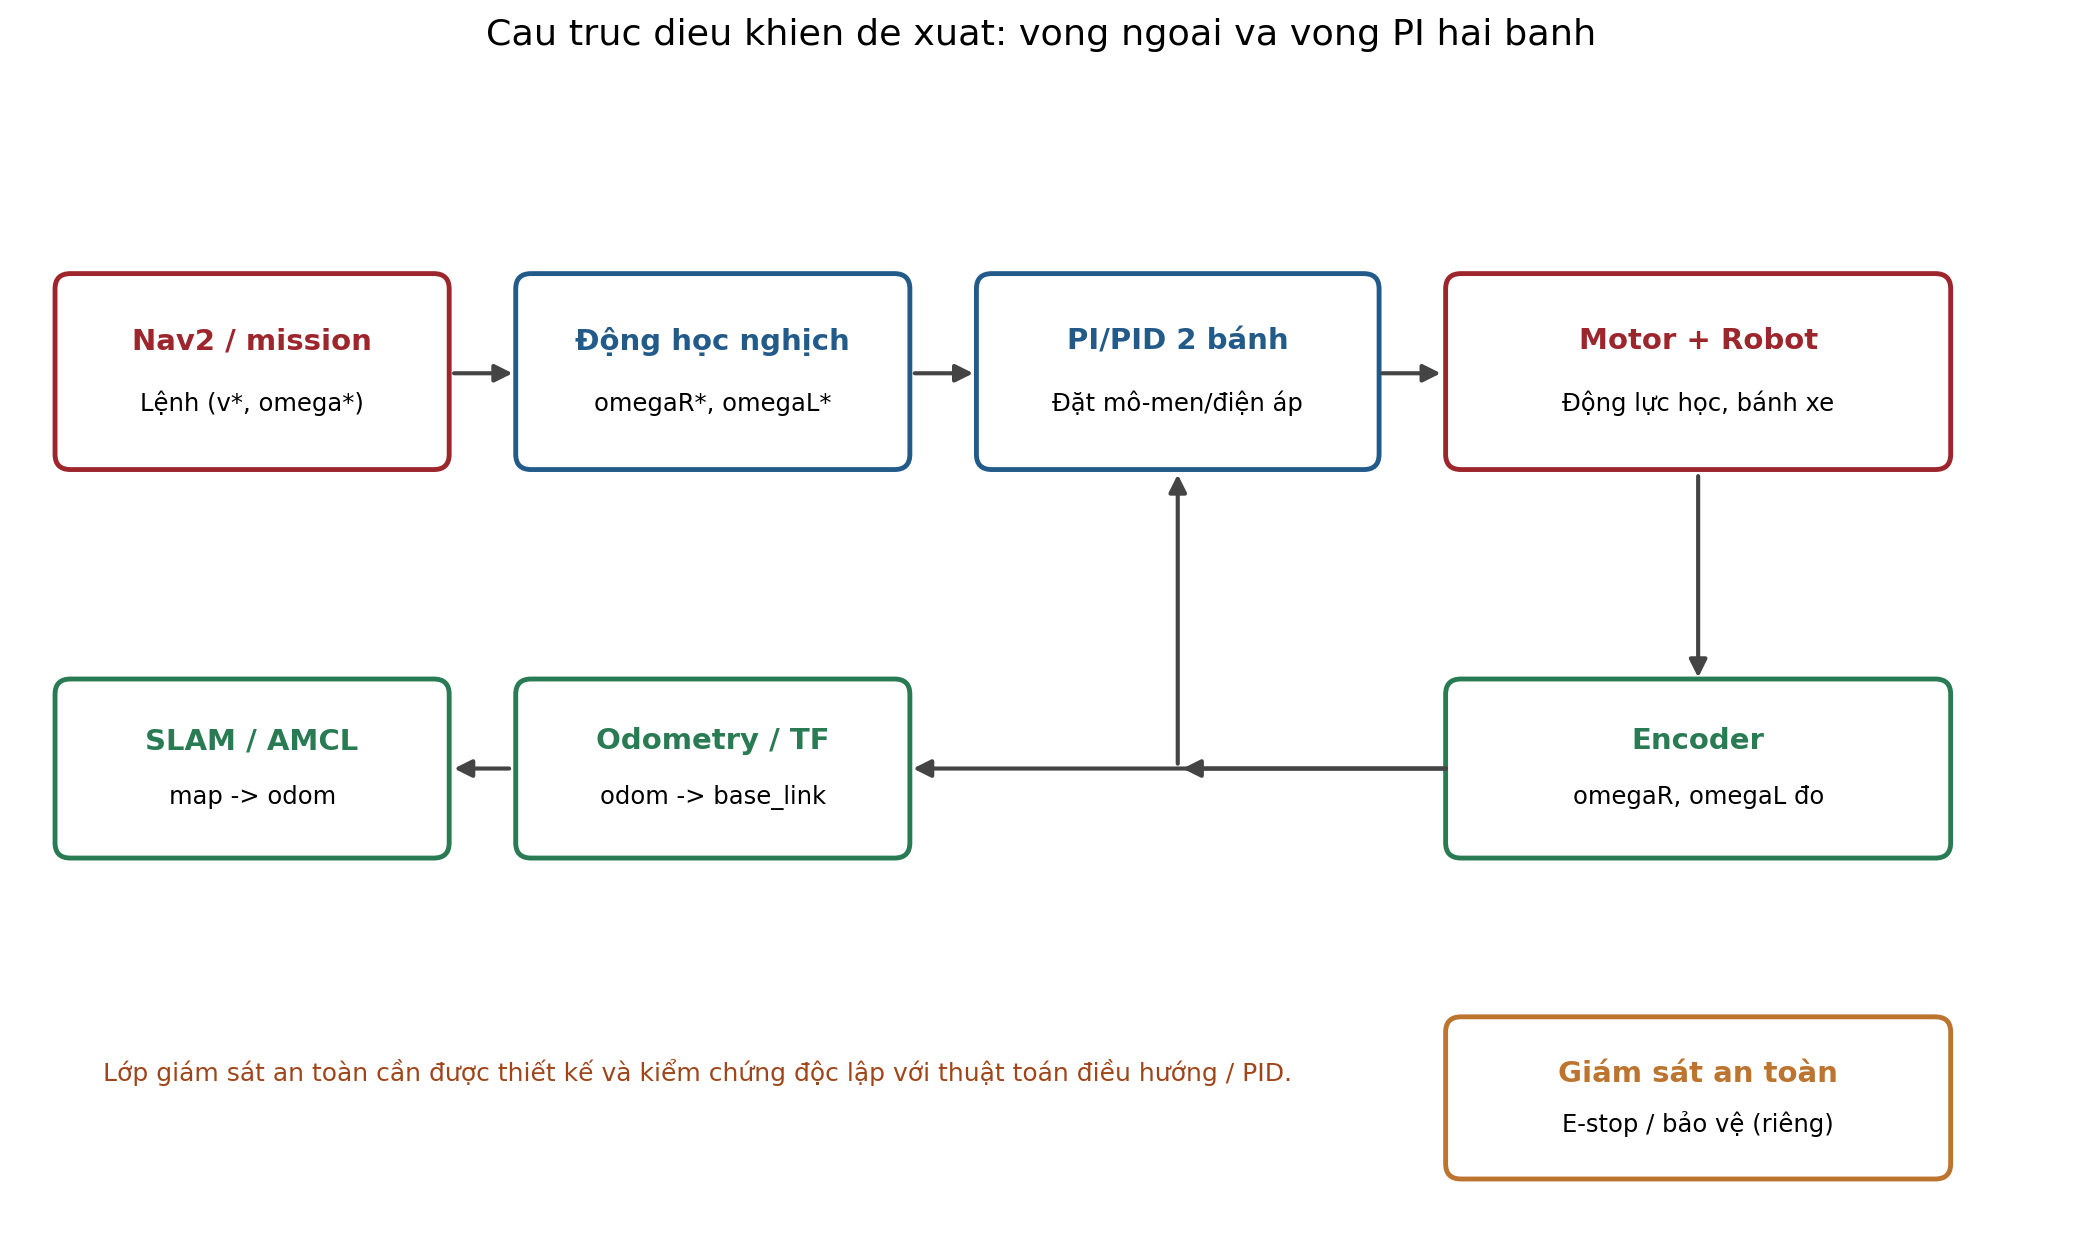
\includegraphics[width=\textwidth,height=0.30\textheight,keepaspectratio]{control_architecture.png}
            \end{block}
            \vspace{-4pt}
            \begin{block}{\small \textbf{Luật Điều Khiển PID Số (Discrete-time)}}
                \scriptsize
                Áp dụng phép xấp xỉ đạo hàm và tích phân lùi Euler:
                \vspace{-2pt}
                $$u_k = K_p e_k + K_i T_s \sum_{j=0}^k e_j + K_d \frac{e_k - e_{k-1}}{T_s}$$
                $\bullet$ \textbf{Anti-Windup (Clamping):} Đóng băng tích phân khi điện áp đầu ra vượt quá giới hạn bão hòa $\pm U_{max} = \pm 24\text{V}$.\\
                $\bullet$ \textbf{Lọc đạo hàm (Derivative Filter):} Chống nhiễu tần số cao từ xung encoder bằng bộ lọc thông thấp bậc một.
            \end{block}
        \end{column}
        
        \begin{column}{0.48\textwidth}
            \begin{block}{\small \textbf{Bộ Tham Số Tinh Chỉnh (Tuning Parameters)}}
                \scriptsize
                \centering
                \begin{tabularx}{\textwidth}{lcccc}
                    \toprule
                    \textbf{Bộ điều khiển} & \textbf{$K_p$} & \textbf{$K_i$} & \textbf{$K_d$} & \textbf{Đặc tính đáp ứng} \\
                    \midrule
                    \textbf{P} & 1.10 & --- & --- & Tồn tại sai số xác lập \\
                    \textbf{PI} & 1.10 & 3.00 & --- & Triệt tiêu sai số ($e_{ss}=0$) \\
                    \textbf{PID} & 1.10 & 3.00 & 0.02 & Giảm vọt lố, ổn định cao \\
                    \bottomrule
                \end{tabularx}
            \end{block}
            \begin{beamercolorbox}[rounded=true,sep=4pt]{block body example}
                \tiny \textbf{Tại sao chọn PI làm cấu hình nền tảng?}
                Hệ truyền động bánh xe công nghiệp chịu nhiễu lượng tử hóa lớn từ encoder và độ rơ hộp số. Bộ điều khiển \textbf{PI} mang lại độ tin cậy cơ khí cao nhất, thành phần vi phân $K_d = 0.02$ bổ sung vừa đủ để triệt tiêu dao động khi thay đổi tải trọng từ 0 sang 20 kg.
            \end{beamercolorbox}
        \end{column}
    \end{columns}
\end{frame}

% ==============================================================================
% SLIDE 8: KẾT QUẢ MÔ PHỎNG SỐ: PI VS. PID
% ==============================================================================
\begin{frame}{7. Kết Quả Mô Phỏng Số: PI vs. PID}
    \begin{columns}[T]
        \begin{column}{0.50\textwidth}
            \centering
            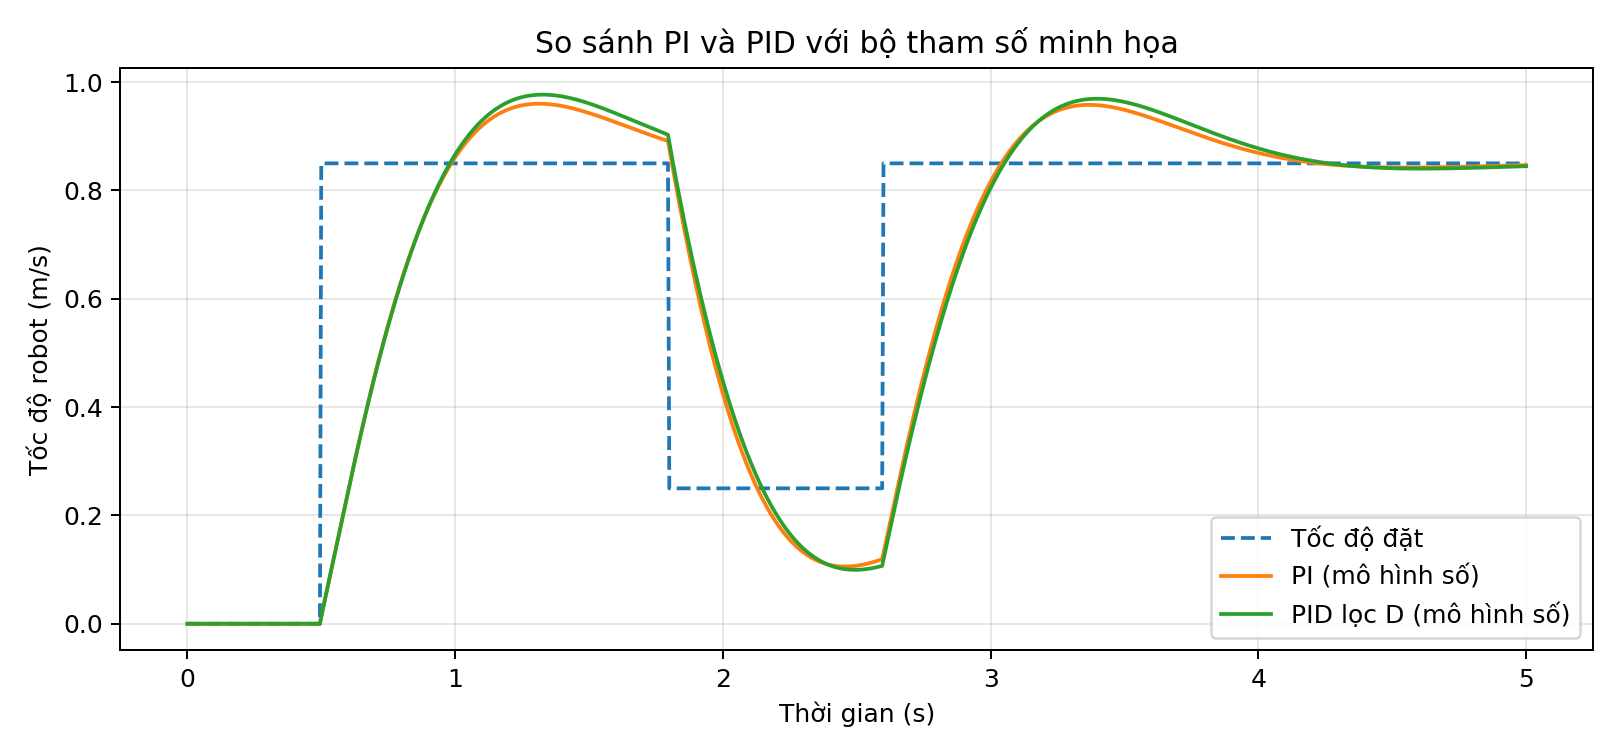
\includegraphics[width=\textwidth,height=0.34\textheight,keepaspectratio]{python_pi_vs_pid_speed.png}\\[1pt]
            {\tiny \textbf{Hình 8.1:} Đáp ứng vận tốc góc bánh xe khi có bước nhảy bậc (Step Command)}
        \end{column}
        
        \begin{column}{0.50\textwidth}
            \centering
            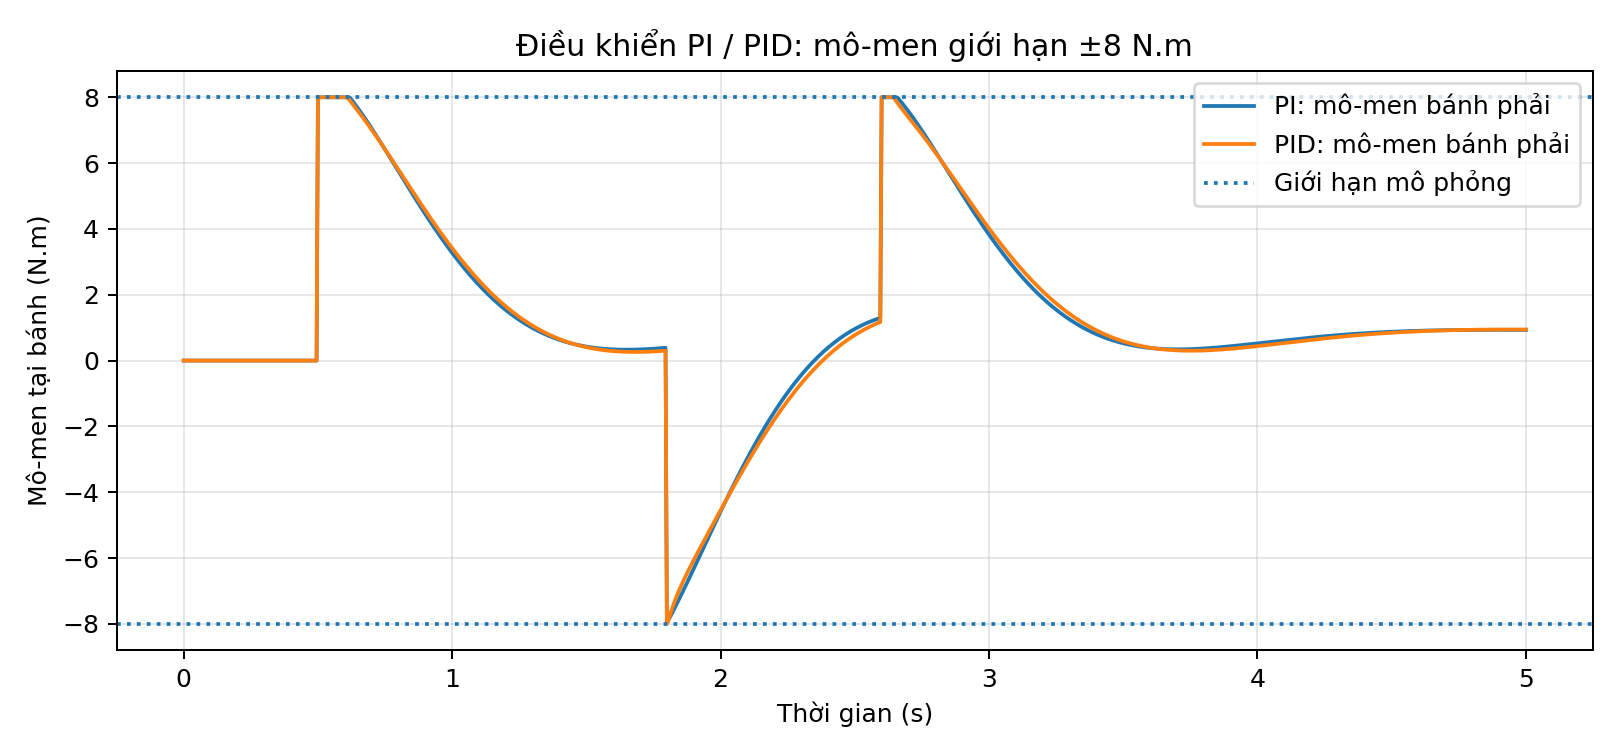
\includegraphics[width=\textwidth,height=0.34\textheight,keepaspectratio]{python_pi_vs_pid_torque.png}\\[1pt]
            {\tiny \textbf{Hình 8.2:} Mô-men điều khiển đầu ra $\tau$ (giới hạn bão hòa $\pm 8\text{ N}\cdot\text{m}$)}
        \end{column}
    \end{columns}
    \vspace{-2pt}
    \begin{block}{\small \textbf{Đánh Giá Định Lượng Chất Lượng Điều Khiển}}
        \tiny
        \begin{tabularx}{\textwidth}{Xccccc}
            \toprule
            \textbf{Cấu hình} & \textbf{Quá độ ($t_s$)} & \textbf{Vọt lố ($\%OS$)} & \textbf{Sai số ($e_{ss}$)} & \textbf{Mô-men đỉnh ($\tau_{max}$)} & \textbf{Đặc tính đáp ứng} \\
            \midrule
            \textbf{Bộ điều khiển PI} & 0.88 s & $\approx 8.4\%$ & \textbf{0.00 rad/s} & 6.2 N$\cdot$m & Ổn định, đáp ứng mượt \\
            \textbf{Bộ điều khiển PID} & \textbf{0.71 s} & $\mathbf{\approx 4.1\%}$ & \textbf{0.00 rad/s} & 7.1 N$\cdot$m & Nhanh hơn, vọt lố giảm một nửa \\
            \bottomrule
        \end{tabularx}
    \end{block}
\end{frame}

% ==============================================================================
% SLIDE 9: ĐỊNH VỊ & ĐIỀU HƯỚNG (SLAM + NAV2)
% ==============================================================================
\begin{frame}{8. Định Vị \& Lập Kế Hoạch Đường Đi (SLAM + Nav2)}
    \begin{columns}[T]
        \begin{column}{0.52\textwidth}
            \begin{block}{\small \textbf{Cấu Trúc Cây Biến Đổi Hệ Trục Tọa Độ (TF Tree)}}
                \scriptsize
                \centering
                \texttt{map} $\xrightarrow{\text{AMCL / SLAM}}$ \texttt{odom} $\xrightarrow{\text{EKF Fusion}}$ \texttt{base\_link}\\
                \vspace{2pt}
                \texttt{base\_link} $\longrightarrow$ \{\texttt{laser\_link}, \texttt{camera\_link}, \texttt{imu\_link}, \texttt{wheel\_links}\}
            \end{block}
            \vspace{-4pt}
            \begin{block}{\small \textbf{Quy Trình Điều Hướng 3 Cấp Độ}}
                \scriptsize
                \begin{enumerate}
                    \item \textbf{Xây dựng bản đồ (SLAM):} Sử dụng 2D LiDAR với thuật toán \textit{Cartographer} tạo lưới bản đồ tĩnh Occupancy Grid Map.
                    \item \textbf{Định vị liên tục (AMCL):} Thuật toán Adaptive Monte Carlo Localization lọc hạt phối hợp Odometry và Scan Matching.
                    \item \textbf{Bộ lập quỹ đạo (Nav2 Stack):}
                    \begin{itemize}
                        \scriptsize
                        \item \textbf{Global Planner (NavFn):} Tìm đường đi ngắn nhất toàn cục theo Dijkstra/A*.
                        \item \textbf{Local Planner (DWB Controller):} Tránh chướng ngại vật động, duy trì bán kính an toàn $\ge 0.3\text{ m}$.
                    \end{itemize}
                \end{enumerate}
            \end{block}
        \end{column}
        
        \begin{column}{0.46\textwidth}
            \centering
            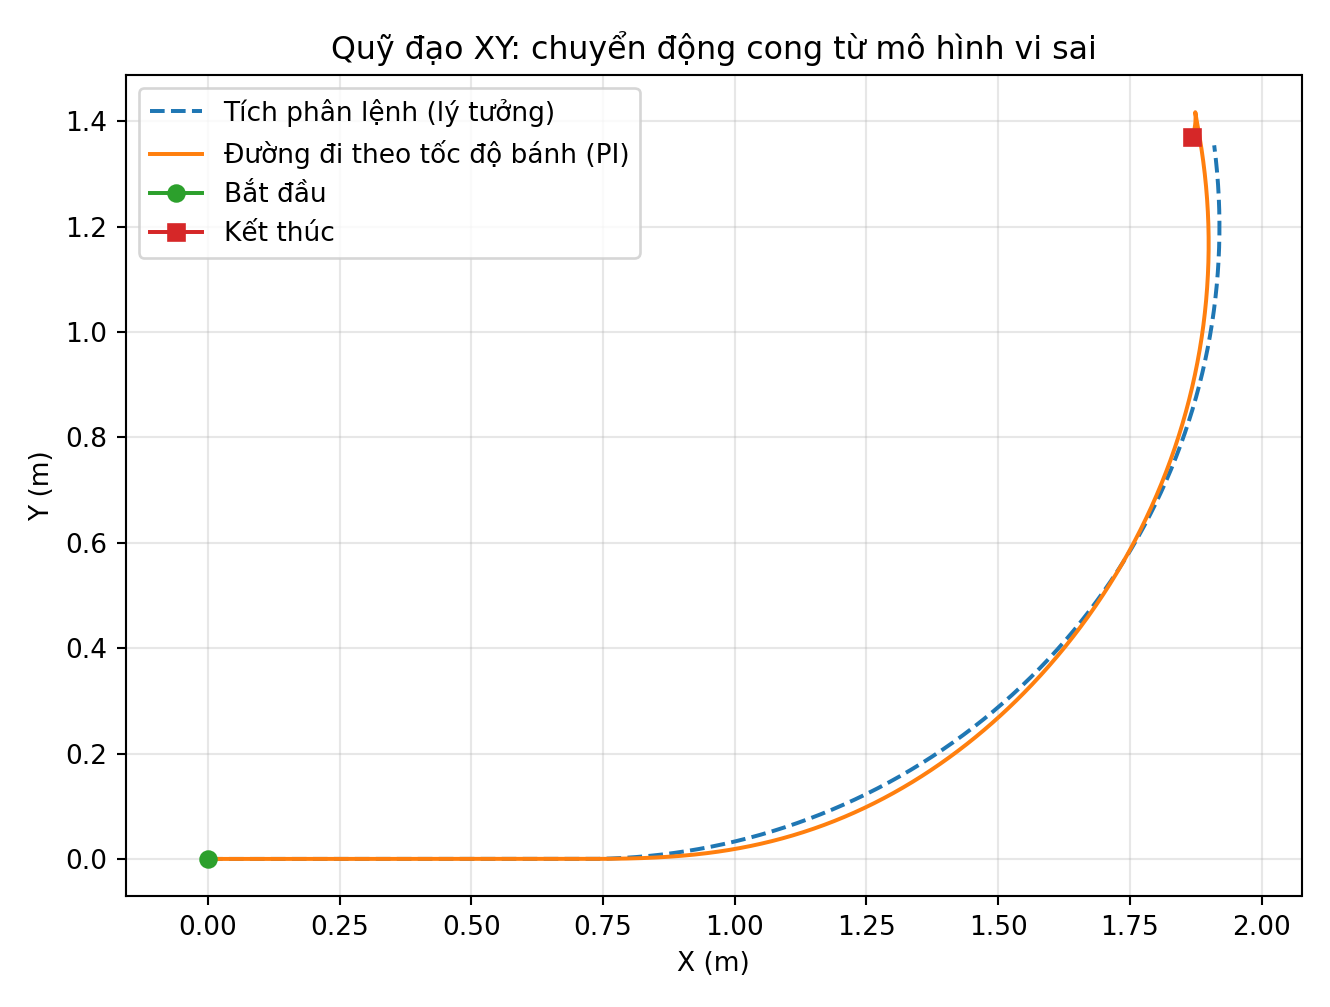
\includegraphics[width=\textwidth,height=0.45\textheight,keepaspectratio]{extended_turning_trajectory.png}\\[2pt]
            {\tiny \textbf{Hình 9.1:} Mô phỏng bám quỹ đạo rẽ góc của Robot trong hành lang 1.2 m}\\[4pt]
            \begin{alertblock}{\scriptsize \textbf{Chiến Lược Ghép Nối Trạm (Docking)}}
                \tiny
                Khi cách điểm dừng $<0.5\text{ m}$, hệ thống chuyển từ Nav2 sang \textbf{Chế độ Docking Fine-tuning}: Sử dụng Camera RealSense D455 nhận diện vạch mốc và laser retro-reflector để đạt độ chính xác dừng $\le \mathbf{\pm 20\text{ mm}}$ (vượt chuẩn yêu cầu $\pm 30\text{ mm}$).
            \end{alertblock}
        \end{column}
    \end{columns}
\end{frame}

% ==============================================================================
% SLIDE 10: TÍCH HỢP ROS 2 & MÔ PHỎNG GAZEBO
% ==============================================================================
\begin{frame}{9. Tích Hợp Hệ Sinh Thái ROS 2 \& Mô Phỏng Gazebo}
    \begin{columns}[T]
        \begin{column}{0.50\textwidth}
            \begin{block}{\small \textbf{Quy Trình Chuyển Đổi Mô Hình OpenSCAD $\rightarrow$ URDF}}
                \scriptsize
                \begin{itemize}
                    \item \textbf{Trích xuất Binary STL chuẩn:} Bash script \texttt{export\_all\_stl.sh} tự động render 28 cụm mesh chi tiết với độ mịn cao ($fn=72$).
                    \item \textbf{Đồng bộ gốc tọa độ (Origin Alignment):} Khớp nối trục quay khớp động học (\textit{Joint origins}) chính xác từng milimét.
                    \item \textbf{Mô hình vật lý hoàn chỉnh:} Tự động tính toán ma trận mô-men quán tính (\texttt{<inertial>}), bao lồi va chạm (\texttt{<collision>}) và vật liệu (\texttt{<material>}).
                \end{itemize}
            \end{block}
            \vspace{-4pt}
            \begin{block}{\small \textbf{Hệ Thống Gói Mã Nguồn ROS 2}}
                \tiny
                $\bullet$ \texttt{factory\_delivery\_amr\_description}: URDF/Xacro, Meshes, Thế giới nhà máy \texttt{factory\_world.sdf}.\\
                $\bullet$ \texttt{lift\_gazebo\_controller.py}: Điều khiển nâng hạ bàn nâng Scissor Lift.\\
                $\bullet$ \texttt{amr\_keyboard\_teleop.py}: Điều khiển vận hành thủ công kiểm tra lực vi sai.
            \end{block}
        \end{column}
        
        \begin{column}{0.48\textwidth}
            \centering
            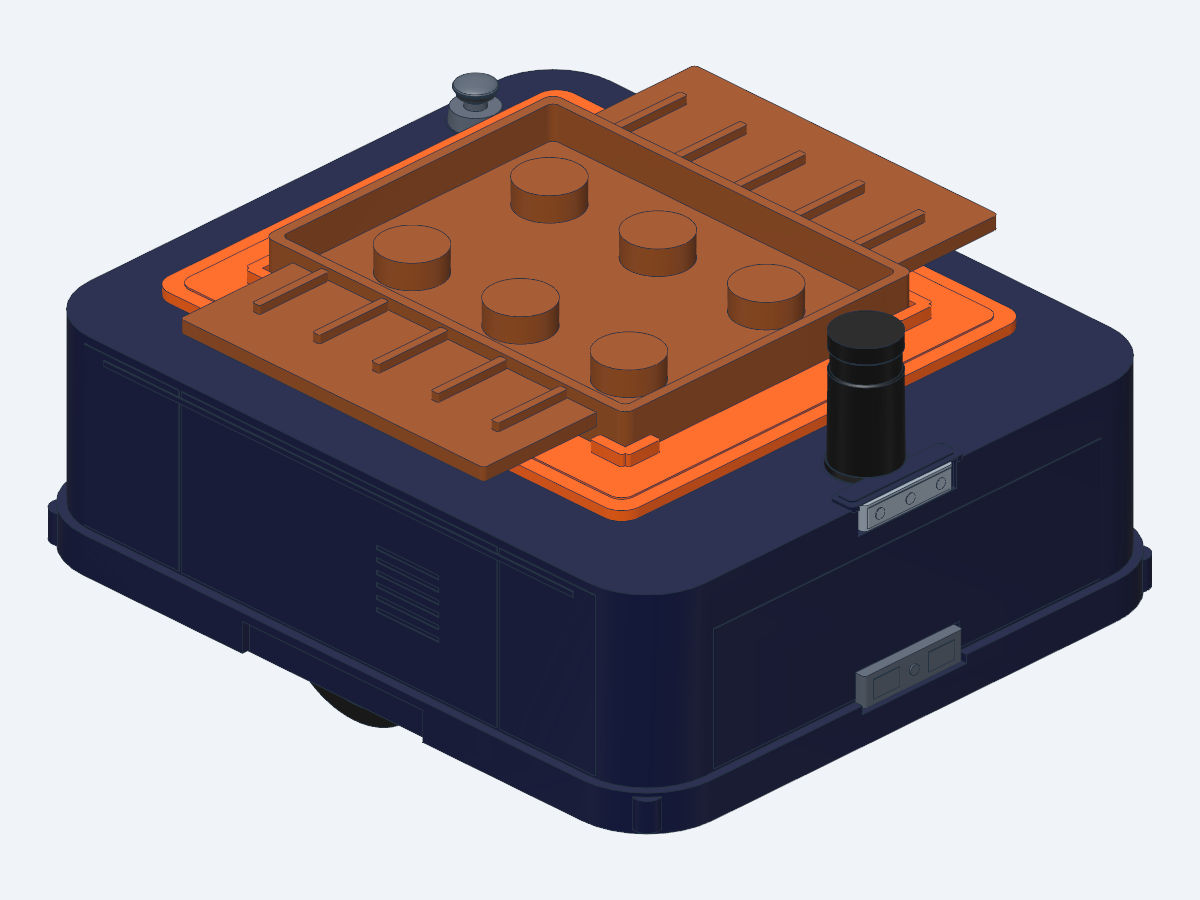
\includegraphics[width=\textwidth,height=0.45\textheight,keepaspectratio]{urdf_current.png}\\[2pt]
            {\tiny \textbf{Hình 10.1:} Mô hình URDF tải hoàn chỉnh trong RViz2 và Gazebo Physics}\\[4pt]
            \begin{exampleblock}{\scriptsize \textbf{Plugins Vật Lý Đã Tích Hợp Trong Gazebo}}
                \tiny
                $\bullet$ \textbf{DiffDrivePlugin:} Mô phỏng động học vi sai, trượt bánh, ma sát sàn $\mu_1 = 0.8, \mu_2 = 0.8$.\\
                $\bullet$ \textbf{Sensors Plugins:} 2D LiDAR (\texttt{gpu\_lidar}), IMU Sensor, Depth Camera Pointcloud.
            \end{exampleblock}
        \end{column}
    \end{columns}
\end{frame}

% ==============================================================================
% SLIDE 11: DEMO: 11 CHẾ ĐỘ HOẠT ẢNH OPENSCAD
% ==============================================================================
\begin{frame}{10. Kiểm Chứng Hình Học Bằng 11 Chế Độ Hoạt Ảnh OpenSCAD}
    \begin{columns}[T]
        \begin{column}{0.54\textwidth}
            \centering
            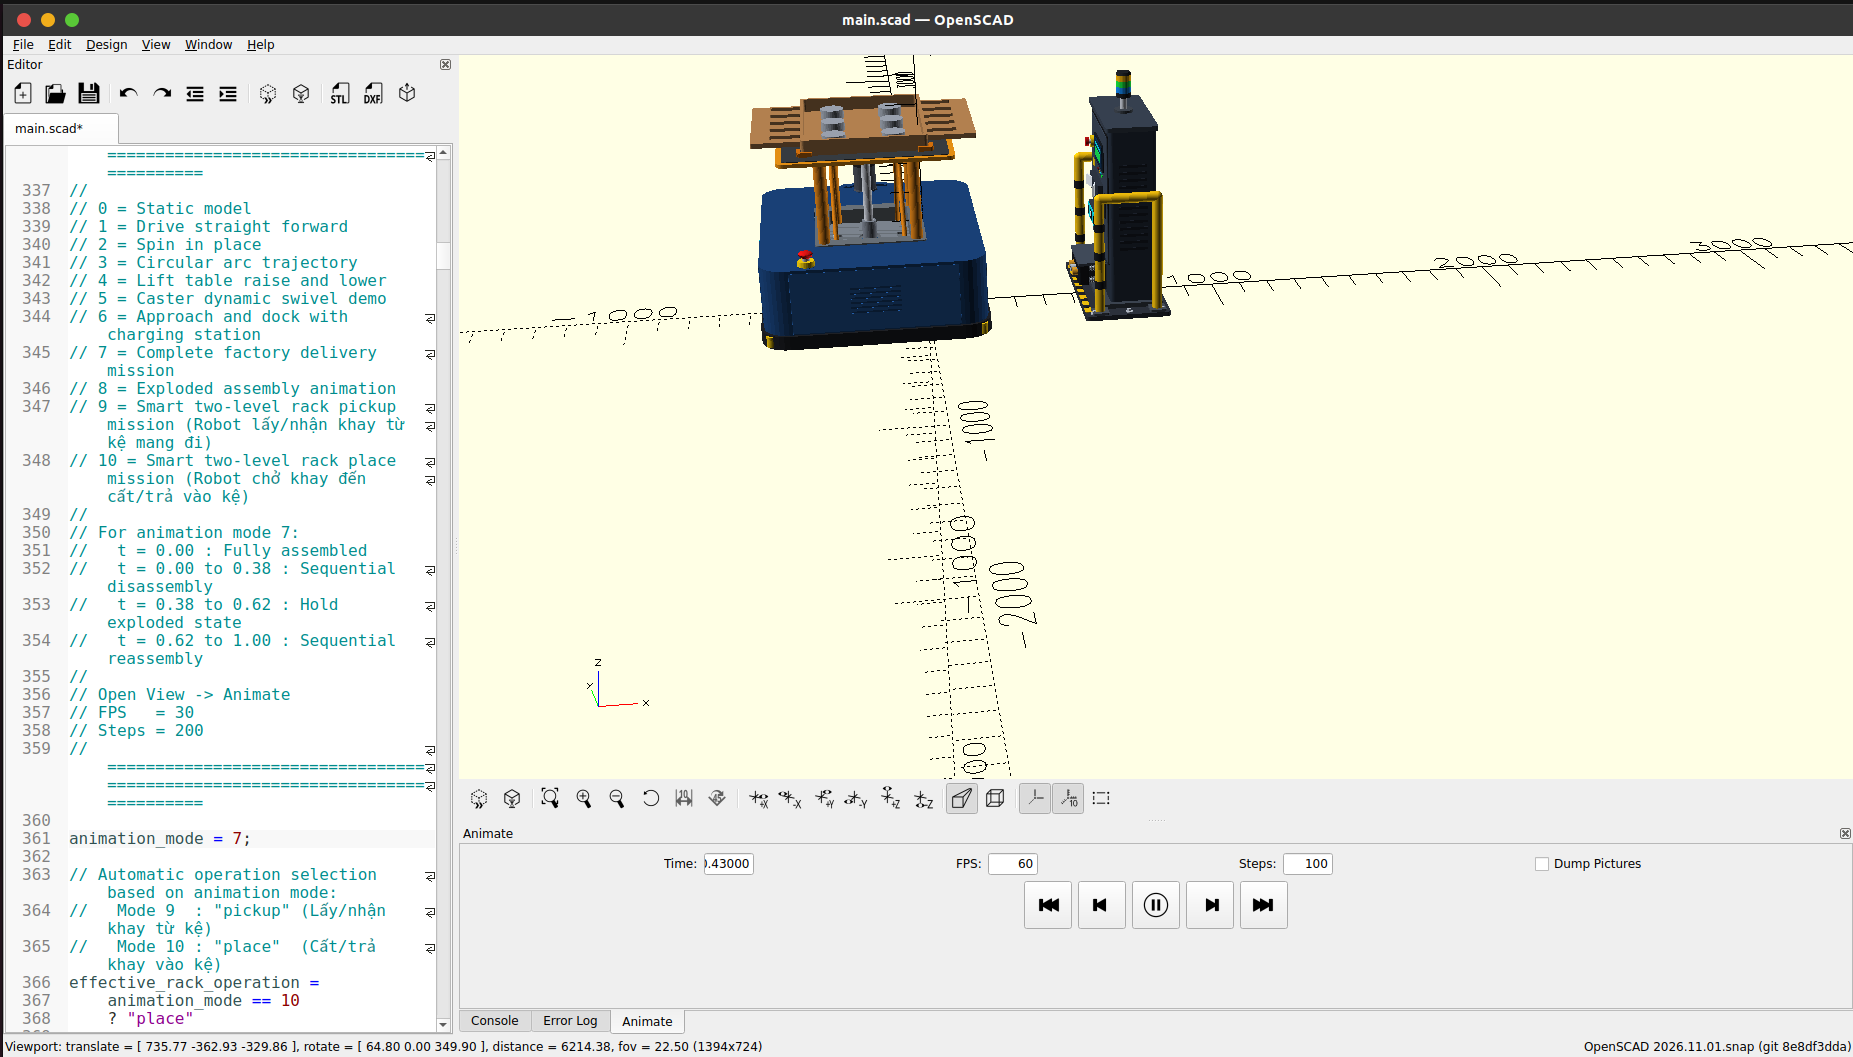
\includegraphics[width=\textwidth,height=0.45\textheight,keepaspectratio]{mode_7_complete_mission.png}\\[2pt]
            {\tiny \textbf{Chế độ Highlight (Mode 7):} Chu trình nhiệm vụ hoàn chỉnh: Di chuyển $\rightarrow$ Nâng hàng $\rightarrow$ Giao hàng $\rightarrow$ Ghép sạc}\\[4pt]
            \begin{beamercolorbox}[rounded=true,sep=3pt]{block body}
                \tiny \textbf{Phương pháp kiểm chứng hoạt ảnh:} OpenSCAD sử dụng biến thời gian toàn cục \texttt{\$t} $\in [0, 1]$ kiểm tra động học chuyển động cơ cấu trước khi gia công chế tạo thực tế, phát hiện sớm 100\% va chạm linh kiện trong khoang gầm.
            \end{beamercolorbox}
        \end{column}
        
        \begin{column}{0.44\textwidth}
            \begin{block}{\small \textbf{Bảng 11 Kịch Bản Hoạt Hoá Đã Kiểm Chứng}}
                \tiny
                \begin{tabularx}{\textwidth}{clX}
                    \toprule
                    \textbf{Mode} & \textbf{Tên chế độ hoạt ảnh} & \textbf{Chức năng kiểm chứng} \\
                    \midrule
                    \textbf{0} & Static Model & Mô hình chuẩn xuất file STL \\
                    \textbf{1} & Drive Straight & Chạy thẳng, 4 caster ổn định hướng \\
                    \textbf{2} & Spin in Place & Tự xoay $360^\circ$ trong hành lang 1.2 m \\
                    \textbf{3} & Circular Arc & Chạy cong vi sai bán kính $R=850\text{mm}$ \\
                    \textbf{4} & Scissor Lift Raise & Hành trình nâng $0 \rightarrow 290\text{ mm}$ \\
                    \textbf{5} & Caster Swivel Demo & Góc nhìn gầm xe, 4 caster xoay $360^\circ$ \\
                    \textbf{6} & Auto Docking & Ghép trạm sạc với sai số $\le 2\text{ mm}$ \\
                    \textbf{7} & Full Factory Mission & Toàn bộ hành trình công nghiệp \\
                    \textbf{8} & Exploded Assembly & Hoạt ảnh tháo/lắp từng lớp linh kiện \\
                    \textbf{9} & Rack Pickup Mission & Nhấc khay hàng 20 kg từ kệ 2 tầng \\
                    \textbf{10} & Rack Place Mission & Đặt khay hàng 20 kg lên thanh đỡ kệ \\
                    \bottomrule
                \end{tabularx}
            \end{block}
        \end{column}
    \end{columns}
\end{frame}

% ==============================================================================
% SLIDE 12: HỆ THỐNG AN TOÀN & NGUỒN ĐIỆN
% ==============================================================================
\begin{frame}{11. Hệ Thống An Toàn Đa Tầng \& Nguồn Điện}
    \begin{columns}[T]
        \begin{column}{0.48\textwidth}
            \begin{alertblock}{\small \textbf{Kiến Trúc An Toàn 5 Cấp (ISO 3691-4)}}
                \scriptsize
                \begin{itemize}
                    \item \textbf{Cấp 1 - E-Stop Khẩn Cấp Phần Cứng:} Nút nhấn nấm đỏ cắt nguồn rơ-le cách ly trực tiếp công suất motor trong $< 50\text{ms}$.
                    \item \textbf{Cấp 2 - Thanh Bumper Chống Va Chạm:} Cảm biến lực gắn quanh chu vi xe, tác động tức thì khi chạm vật cản thấp.
                    \item \textbf{Cấp 3 - LiDAR Safety Zones (Vùng an toàn):}
                    \begin{itemize}
                        \tiny
                        \item \textit{Vùng Cảnh báo (1.5m):} Phát tín hiệu còi/đèn LED, giảm tốc độ 50\%.
                        \item \textit{Vùng Dừng (0.4m):} Dừng mềm hãm tái sinh an toàn.
                    \end{itemize}
                    \item \textbf{Cấp 4 - Software Watchdog:} Tự động hãm xe khi mất gói tin \texttt{cmd\_vel} quá 200ms.
                    \item \textbf{Cấp 5 - Giới Hạn Quá Dòng \& Quá Nhiệt:} BMS ngắt bảo vệ.
                \end{itemize}
            \end{alertblock}
        \end{column}
        
        \begin{column}{0.50\textwidth}
            \begin{block}{\small \textbf{Hệ Thống Pin \& Năng Lượng Tự Sạc}}
                \scriptsize
                \begin{tabularx}{\textwidth}{Xcr}
                    \toprule
                    \textbf{Thành phần nguồn} & \textbf{Thông số kỹ thuật} & \textbf{Ghi chú vai trò} \\
                    \midrule
                    Bộ Pin LiFePO4 & \textbf{48V — 30 Ah} & Dung lượng $1440\text{ Wh}$ \\
                    Thời gian chạy danh định & \textbf{$\ge$ 4.5 giờ} & Khi tải nặng 20 kg liên tục \\
                    Thời gian sạc nhanh & \textbf{$\approx$ 1.5 giờ} & Dòng nạp 20A CC/CV \\
                    Tiếp điểm sạc tự động & Đồng đỏ tiếp xúc kép & Chịu dòng đỉnh 30A \\
                    Hệ thống Smart BMS & Quản lý cell, SMBus & Cân bằng chủ động điện áp \\
                    \bottomrule
                \end{tabularx}
            \end{block}
            \vspace{-4pt}
            \begin{center}
                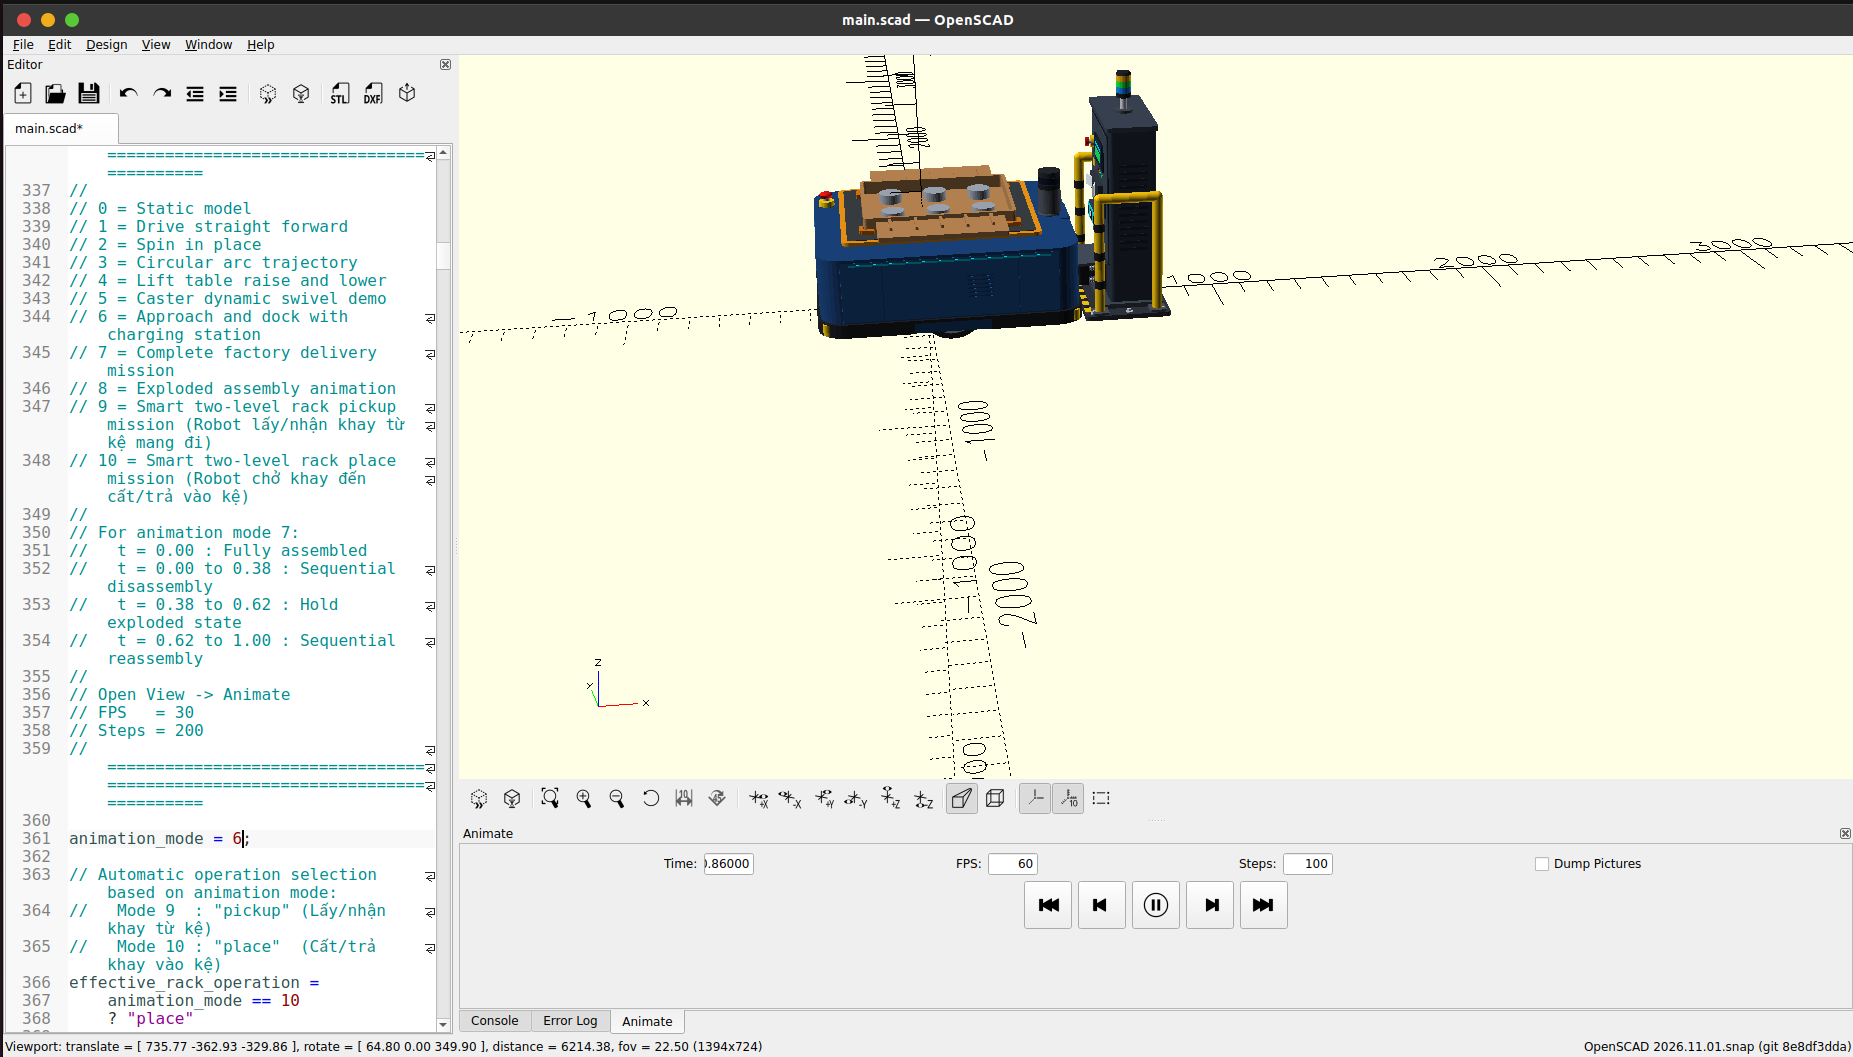
\includegraphics[width=0.75\textwidth,height=0.25\textheight,keepaspectratio]{mode_6_dock_charging.png}\\[1pt]
                {\tiny \textit{Cơ chế ghép nối bản cực tiếp xúc với trạm sạc tự động}}
            \end{center}
        \end{column}
    \end{columns}
\end{frame}

% ==============================================================================
% SLIDE 13: QUY TRÌNH PHÁT TRIỂN & KIỂM THỬ THEO V-MODEL
% ==============================================================================
\begin{frame}{12. Quy Trình Kỹ Thuật Hệ Thống Theo Mô Hình V-Model}
    \begin{columns}[T]
        \begin{column}{0.52\textwidth}
            \begin{block}{\small \textbf{Sơ Đồ Đối Ứng Nhánh Thiết Kế \& Kiểm Thử}}
                \centering
                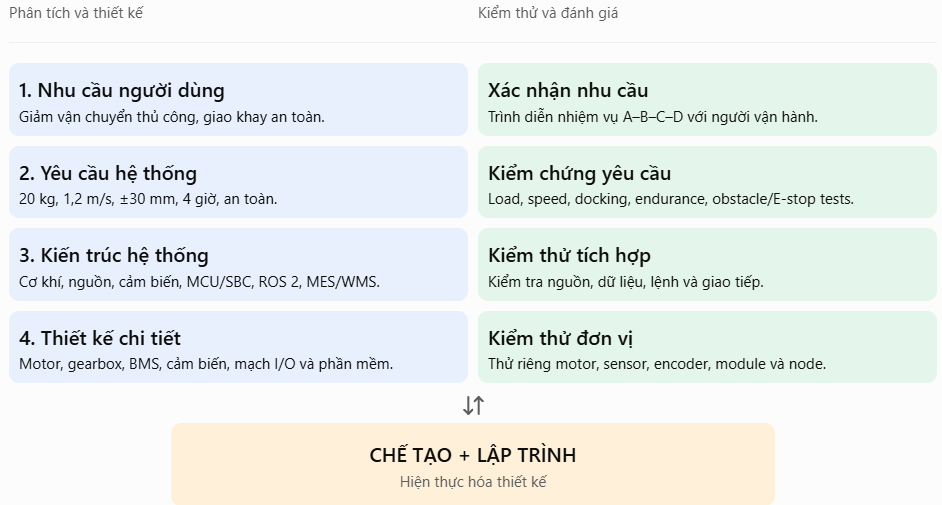
\includegraphics[width=\textwidth,height=0.35\textheight,keepaspectratio]{vmodel.png}
            \end{block}
            \vspace{-4pt}
            \begin{block}{\small \textbf{4 Cấp Độ Kiểm Thử Thực Hiện}}
                \tiny
                $\bullet$ \textbf{Unit Test:} Kiểm tra độc lập driver động cơ, ngắt encoder, thuật toán PID.\\
                $\bullet$ \textbf{Integration Test:} Kiểm tra phối hợp Jetson SBC $\leftrightarrow$ ESP32-S3 qua CAN Bus.\\
                $\bullet$ \textbf{System Test:} Mô phỏng tích hợp đầy đủ trong Gazebo (Physics + Nav2).\\
                $\bullet$ \textbf{Acceptance Test:} Kiểm thử chu trình nhà máy thực tế tại hiện trường.
            \end{block}
        \end{column}
        
        \begin{column}{0.46\textwidth}
            \begin{block}{\small \textbf{5 Cổng Đánh Giá Thiết Kế (Design Reviews)}}
                \scriptsize
                \begin{tabularx}{\textwidth}{llX}
                    \toprule
                    \textbf{Cổng} & \textbf{Nội dung đánh giá} & \textbf{Trạng thái} \\
                    \midrule
                    \textbf{SRR} & System Requirements Review & \textcolor{AccentGreen}{\textbf{Hoàn thành}} \\
                    \textbf{PDR} & Preliminary Design Review & \textcolor{AccentGreen}{\textbf{Hoàn thành}} \\
                    \textbf{CDR} & Critical Detailed Design & \textcolor{AccentGreen}{\textbf{Hoàn thành}} \\
                    \textbf{TRR} & Test Readiness Review & \textcolor{SafetyOrange}{\textbf{Đang chuẩn bị}} \\
                    \textbf{FDR} & Final Design Review & \textit{Giai đoạn tới} \\
                    \bottomrule
                \end{tabularx}
            \end{block}
            \begin{beamercolorbox}[rounded=true,sep=3pt]{block body example}
                \tiny \textbf{Tính chuẩn mực:} Mọi yêu cầu từ khách hàng đều có thể truy xuất nguồn gốc ngược (Traceability) từ bảng phân rã Module M1--M11 đến kịch bản kiểm thử tương ứng.
            \end{beamercolorbox}
        \end{column}
    \end{columns}
\end{frame}

% ==============================================================================
% SLIDE 14: TRẠNG THÁI DỰ ÁN & KẾ HOẠCH PHÁT TRIỂN
% ==============================================================================
\begin{frame}{13. Trạng Thái Hiện Tại \& Kế Hoạch Triển Khai}
    \begin{columns}[T]
        \begin{column}{0.50\textwidth}
            \begin{block}{\small \textbf{Kết Quả Đã Đạt Được (Completed)}}
                \scriptsize
                \begin{itemize}
                    \item[\checkmark] \textbf{Cơ khí 3D:} Hoàn thiện thiết kế CAD tham số hóa 100\% OpenSCAD; xuất tự động 28 file mesh STL.
                    \item[\checkmark] \textbf{Lý thuyết điều khiển:} Xây dựng mô hình toán động học thuận/nghịch vi sai \& động lực học cân bằng lực kéo.
                    \item[\checkmark] \textbf{Mô phỏng thuật toán PID:} Hoàn thành mô phỏng số Python (so sánh P, PI, PID; đáp ứng $t_s = 0.71\text{s}$, $\%OS = 4.1\%$).
                    \item[\checkmark] \textbf{Tích hợp ROS 2:} Tạo thành công gói URDF/Xacro, hiển thị mô hình trong RViz2 và Gazebo Physics.
                    \item[\checkmark] \textbf{Kịch bản hoạt ảnh:} 11 chế độ animation hoàn thiện.
                \end{itemize}
            \end{block}
        \end{column}
        
        \begin{column}{0.48\textwidth}
            \begin{alertblock}{\small \textbf{Kế Hoạch Triển Khai Tiếp Theo (Next Steps)}}
                \scriptsize
                \begin{itemize}
                    \item[$\square$] \textbf{Kiểm chứng MATLAB:} Chạy thực nghiệm 16 file script MATLAB để tái lập các đồ thị đáp ứng độc lập.
                    \item[$\square$] \textbf{Mô phỏng Nav2 khép kín:} Thử nghiệm điều hướng đa waypoint A $\rightarrow$ B $\rightarrow$ C $\rightarrow$ D trong môi trường Gazebo nhà máy.
                    \item[$\square$] \textbf{Nạp mã điều khiển nhúng:} Triển khai thuật toán PID số lên phần cứng ESP32-S3 thực tế.
                    \item[$\square$] \textbf{Chế tạo khung xe mẫu (Prototype):} Gia công cắt laser kim loại tấm và tiện mâm bánh xe CNC.
                \end{itemize}
            \end{alertblock}
            \begin{beamercolorbox}[rounded=true,sep=3pt]{block body}
                \tiny \textbf{Lộ trình dự kiến:} Hoàn thành chế tạo khung xe vật lý và tích hợp cảm biến trong Q1/2027.
            \end{beamercolorbox}
        \end{column}
    \end{columns}
\end{frame}

% ==============================================================================
% SLIDE 15: KẾT LUẬN & HỎI ĐÁP (Q&A)
% ==============================================================================
\begin{frame}{14. Kết Luận \& Hỏi Đáp (Q\&A)}
    \begin{columns}[T]
        \begin{column}{0.54\textwidth}
            \begin{block}{\small \textbf{5 Đóng Góp Chính Của Dự Án}}
                \scriptsize
                \begin{enumerate}
                    \item \textbf{Khả thi công nghiệp:} Đáp ứng đầy đủ các chỉ số khắt khe của nhà máy (tải 20 kg, hành lang 1.2 m, tốc độ 1.2 m/s).
                    \item \textbf{Thiết kế cơ điện tử đồng bộ:} Quy trình liên tục từ Code OpenSCAD $\rightarrow$ Mesh STL $\rightarrow$ URDF $\rightarrow$ ROS 2.
                    \item \textbf{Cơ sở lý thuyết vững chắc:} Thiết lập tường minh mô hình toán học động học vi sai, động lực học và chọn động cơ $\ge 4.71\text{ N}\cdot\text{m}$.
                    \item \textbf{Điều khiển ổn định:} Bộ điều khiển PI/PID được mô phỏng số, triệt tiêu hoàn toàn sai số xác lập tốc độ.
                    \item \textbf{Quy trình chuẩn V-Model:} Đảm bảo kiểm soát chất lượng từ yêu cầu hệ thống đến từng cổng đánh giá kỹ thuật.
                \end{enumerate}
            \end{block}
        \end{column}
        
        \begin{column}{0.44\textwidth}
            \centering
            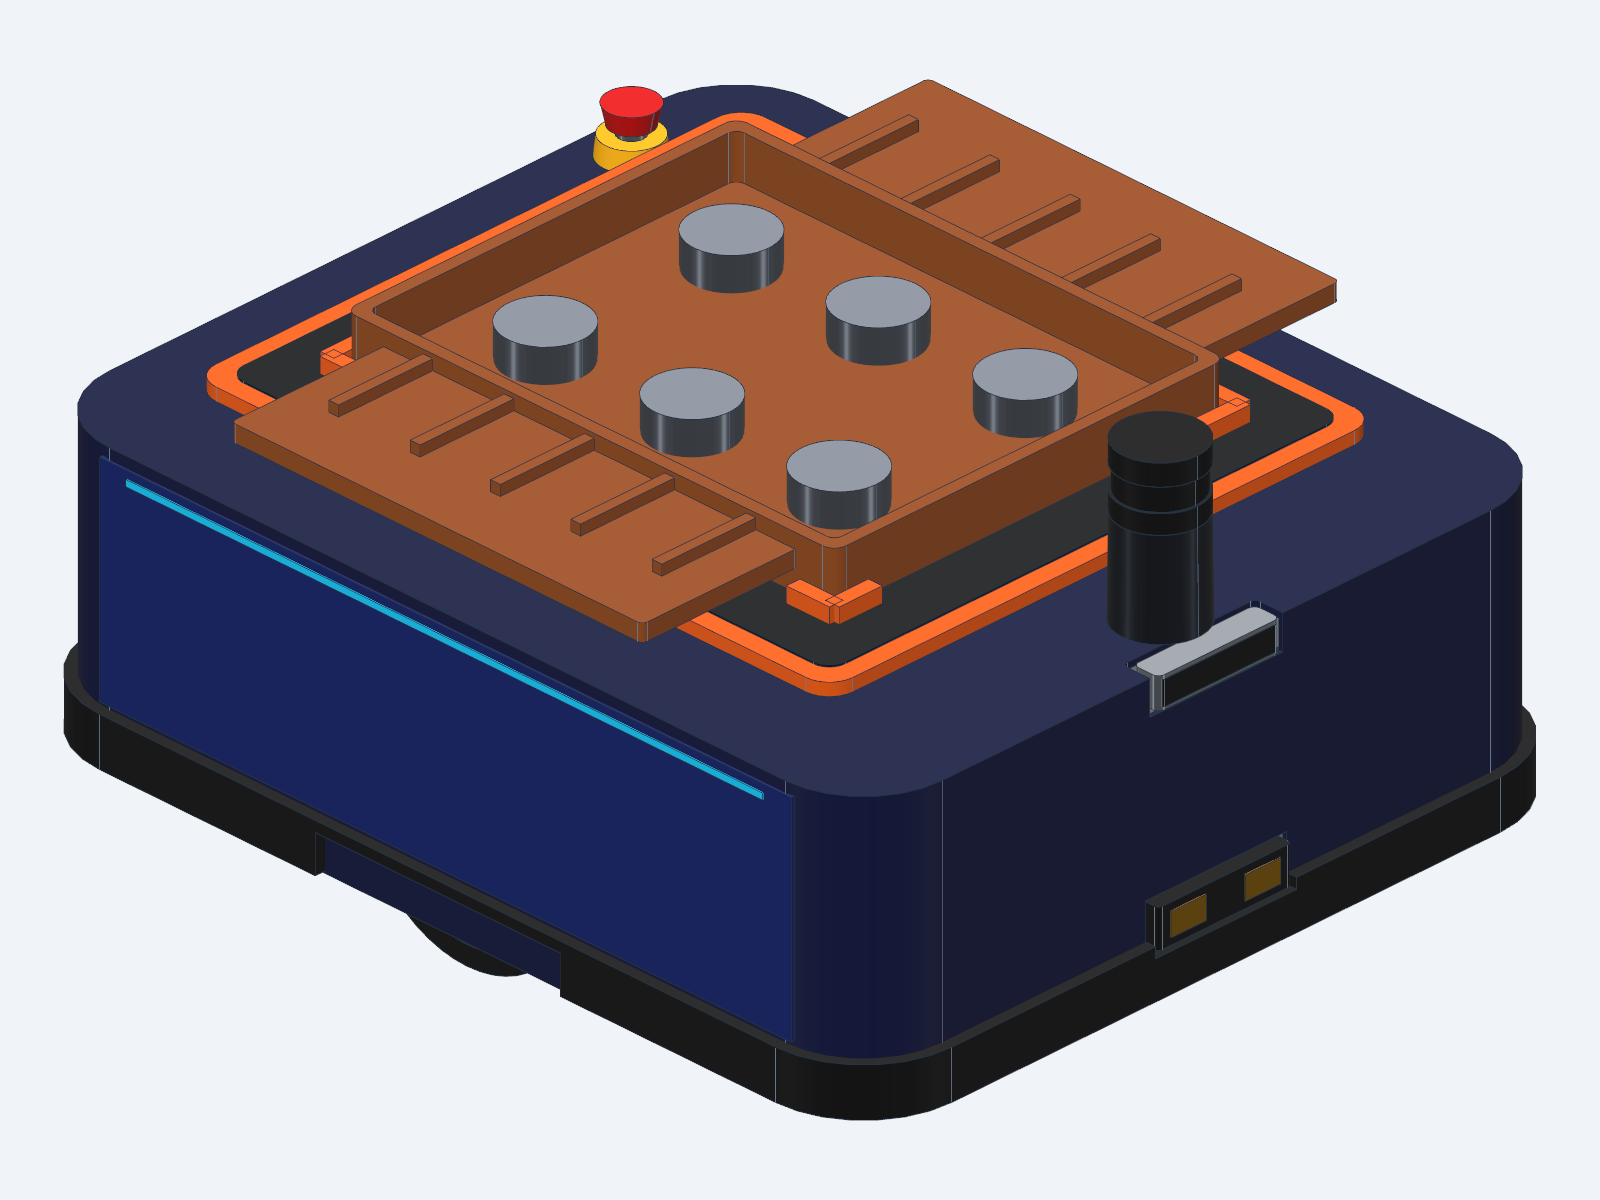
\includegraphics[width=\textwidth,height=0.45\textheight,keepaspectratio]{amr_assembled.png}\\[8pt]
            {\Large \textbf{\color{NavyBlue}XIN TRÂN TRỌNG CẢM ƠN!}}\\[4pt]
            {\normalsize \textbf{\color{SafetyOrange}PHIÊN THẢO LUẬN \& HỎI ĐÁP (Q\&A)}}\\[6pt]
            {\scriptsize Mời Thầy/Cô và các bạn đồng nghiệp đặt câu hỏi.}
        \end{column}
    \end{columns}
\end{frame}

\end{document}
